% BD region of the Assignment 8 chapter (course Chapter 6), rows 4, 5, 6, 7. Written Nov 17, 2026 from evidence 200-239.
% To be placed in devopsDelivery.tex of the Gitea manual repository next to SD's region (rows 1, 2, 3, 8). The evidence files named below
% live in the course repository, assignment-8/evidence, and must be copied into the manual repository's evidence folder for the build.
% Times: UTC is the server clock; US Eastern (EST) is UTC minus 5 hours (Nov 17, 2026 evening in New York is Nov 18 UTC).

% ===== BD region: row 4 (15 points) =====
\section{Jenkins delivery gates, approval and promotion (15 points)}\label{Section:deliveryJenkins}
\textbf{Owner:} BD. \textbf{Status:} v1 and v2 promoted through staging and a named approval on November 17, 2026 (builds \#7 and \#11) \StatusPass.

\paragraph{Capacity before anything was built.} The delivery agent, the scan database and the application images did not fit on the
\texttt{t3.small}. With the team's agreement BD resized the same instance to \texttt{t3.medium} (3,835~MiB of RAM, the same 20~GB disk,
the same Elastic IP, a stop of about 25~seconds) and re-measured (\ListRef{200}). The disk stayed the tight resource: 6.3~GB free before the
delivery work, 3.5~GB after all releases, recoveries and scans (83\% used). The 5.8~GB image of the LaTeX runner and the 1.7~GB Trivy database cannot
be reduced, so the team chose to watch the disk instead of enlarging it; free space is reported after each run, with 2~GB as the stop line.

\paragraph{Trusted agent.} Delivery runs on a separate container, \texttt{jenkins-agent}, built from \texttt{jenkins/inbound-agent} pinned by
digest, with label \texttt{delivery}, one executor, connected over WebSocket (the controller's agent port 50000 stays closed), a memory limit
of 1,536~MiB and no published ports. The node's usage is ``only build jobs with label expressions matching this node'' (\FigRef{206}).
Tools inside it, recorded when it started (\ListRef{205}): Docker CLI 25.0.5, Trivy 0.76.2, ansible-core 2.22.0, pip-audit 2.10.1, Python 3.13.5 and Java 21.
The agent mounts the host's Docker socket, which is root-equivalent on the host; this is an accepted and documented risk. Two incidents while starting
it are kept in the record (\ListRef{205}): the node name was first taken by the connection of BD's own PC (a handshake error on the server side, stopped at once, because the label \texttt{delivery}
is what carries the credentials), and the first node secret was a longer string than the 64 hex characters of a real secret, found by a length and format check without printing it.

\paragraph{Controller changes.} Pull-request builds run only the test stage on the controller. The controller image had no \texttt{pip} or \texttt{venv}, so the hashed install of the
application requirements failed there; BD added \texttt{python3-venv} and \texttt{python3-pip} (image tag \texttt{2.580.2-venv}), recreated the container in about 14~seconds with the
same \texttt{jenkins\_home} volume, and the jobs, plugins and build history were unchanged (\ListRef{202}).

\paragraph{The pipeline.} One \texttt{Jenkinsfile} in the \texttt{twintrack} repository (reviewed in pull requests \#14, \#22 and \#24):
\begin{tabularx}{\linewidth}{L{3.6cm}L{2.7cm}Y}
\caption{Stages of the delivery pipeline\label{Table:DeliveryStages}}\\
\toprule \textbf{Stage} & \textbf{Where} & \textbf{What it does and what blocks}\\ \midrule
\endfirsthead
\toprule \textbf{Stage} & \textbf{Where} & \textbf{What it does and what blocks}\\ \midrule
\endhead \bottomrule \endlastfoot
Tests & controller, every branch & compile and unit tests of the course code, then a hashed install of \texttt{pricing-service/requirements.txt} and the service tests; no credentials, no Docker.\\
Record versions & trusted agent, \texttt{main} only & checkout, clean \texttt{reports/} and untracked records, record the tool versions.\\
Dependency and secret scans & trusted agent & pip-audit on the hashed requirements; Trivy secret scan; a missing report or a non-zero exit stops the build (Section~\ref{Section:deliveryScans}).\\
Build once and scan the image & trusted agent & one image per commit, Trivy image scan for HIGH and CRITICAL, push to the Gitea registry with the write token, digest recorded.\\
Deploy staging & trusted agent & release record, \texttt{ansible-playbook} through the \texttt{deploy} account; health, version, commit and price checks through the public name.\\
Approval & named people & \texttt{input} for \texttt{brahmi} or \texttt{sakshi}, 30-minute timeout; the actual approver is recorded.\\
Deploy production & trusted agent & the same digest, the same playbook, a production record that carries the approval line.\\
\end{tabularx}

Rules written in the file's header and checked in the runs: delivery runs only for \texttt{main}; \texttt{beforeAgent true} so that other builds never take the trusted agent;
\texttt{disableConcurrentBuilds}; credentials are bound only inside the delivery stages and are never put into a Groovy string; one image per commit; the same digest from staging to production.
A pipeline-only or record-only merge builds and deploys nothing: the delivery stage is skipped when the change touches \texttt{releases/} or only \texttt{Jenkinsfile.rollback} (builds \#9 and \#10, the merges of the records pull request and of the rollback fix, \ListRef{223}); the v2 merge, which changes
\texttt{app.py}, ran it (\ListRef{230}).

\paragraph{Approval.} The two Jenkins users are exactly \texttt{brahmi} and \texttt{sakshi} (\FigRef{210}). The prompt names the full digest, the commit and the version (\FigRef{214}); the answer is recorded in the console, in \texttt{reports/approval.txt} and in the production record (\FigRef{215}, \FigRef{217}).

\paragraph{v1 to production (build \#7, commit \texttt{975d13c}).} Tests, scans and image scan passed; staging showed version v1, total 30 for quantity 3; BD approved at 04:36:33~UTC; production received the \emph{same}
digest \texttt{sha256:ce514106\ldots 98b2}; both Ansible runs ended \texttt{ok=9 failed=0} (\ListRef{216}); the URL in a browser (\FigRef{218}).

\paragraph{v2 to production (build \#11, commit \texttt{06550eb}).} Staging showed version v2 and total 36 while production still served v1 (\ListRef{230}); BD promoted at 02:21:44~UTC on November 18 (\FigRef{229}); production container started 13~seconds later,
public checks showed v2 and 36 (\ListRef{231}).

\paragraph{What the runs taught.} (1) Build \#5 failed in 26~seconds: pip-audit could not create its cache because the Trivy volume made \texttt{/home/jenkins/.cache} root-owned; a missing report correctly failed the stage; the agent image
was rebuilt with owned cache directories (\ListRef{212}). (2) The old pull-request workspaces on the agent came from the first Jenkinsfile checking \texttt{when branch main} after allocating the trusted agent; \texttt{beforeAgent true} prevents it (\ListRef{212}).
(3) Build \#7 still held build \#6's scan report in the workspace; \texttt{reports/} is now removed at the start of delivery. (4) The merge of the pipeline change started build \#8, which staged a new digest of the same v1; it was aborted at the approval,
so production never changed, and is listed as ``built and staged, not promoted'' (\ListRef{222}, \FigRef{221}).

\paragraph{Limits, said plainly.} The approval restricts \emph{who} may click, not \emph{what} is correct. A pull-request author can edit the \texttt{Jenkinsfile}; the protection is review before \texttt{main} and the fact that credentials exist only in stages that run for \texttt{main}.
The Docker socket gives the agent root-equivalent power on the host. Jenkins administrators can replay a build with an edited script; this was used on purpose twice (Section~\ref{Section:deliveryRecovery}, Section~\ref{Section:deliveryScans}) and shows in the console as ``Replayed \#n''.
One executor means a build waiting for approval holds the agent for up to 30~minutes.

\begin{longlisting}
\inputminted[fontsize=\scriptsize]{text}{evidence/200-capacity-resize-t3-medium-and-baseline-after-bd-2026-11-12.txt}
\caption{The resize of the instance to \texttt{t3.medium} and the baseline after it, November 12, 2026 (real output).}
\label{Listing:E200}
\end{longlisting}

\begin{longlisting}
\inputminted[fontsize=\scriptsize]{text}{evidence/202-jenkins-controller-image-pip-venv-added-recreated-state-kept-bd-2026-11-12.txt}
\caption{The controller image gets pip and venv; Jenkins recreated with its volume kept (real output).}
\label{Listing:E202}
\end{longlisting}

\begin{longlisting}
\inputminted[fontsize=\scriptsize]{text}{evidence/205-trusted-agent-built-started-connected-bd-2026-11-13.txt}
\caption{The trusted agent: image build, start, connection, tool versions and the incidents (real output).}
\label{Listing:E205}
\end{longlisting}

\begin{figure}[htbp]
\centering
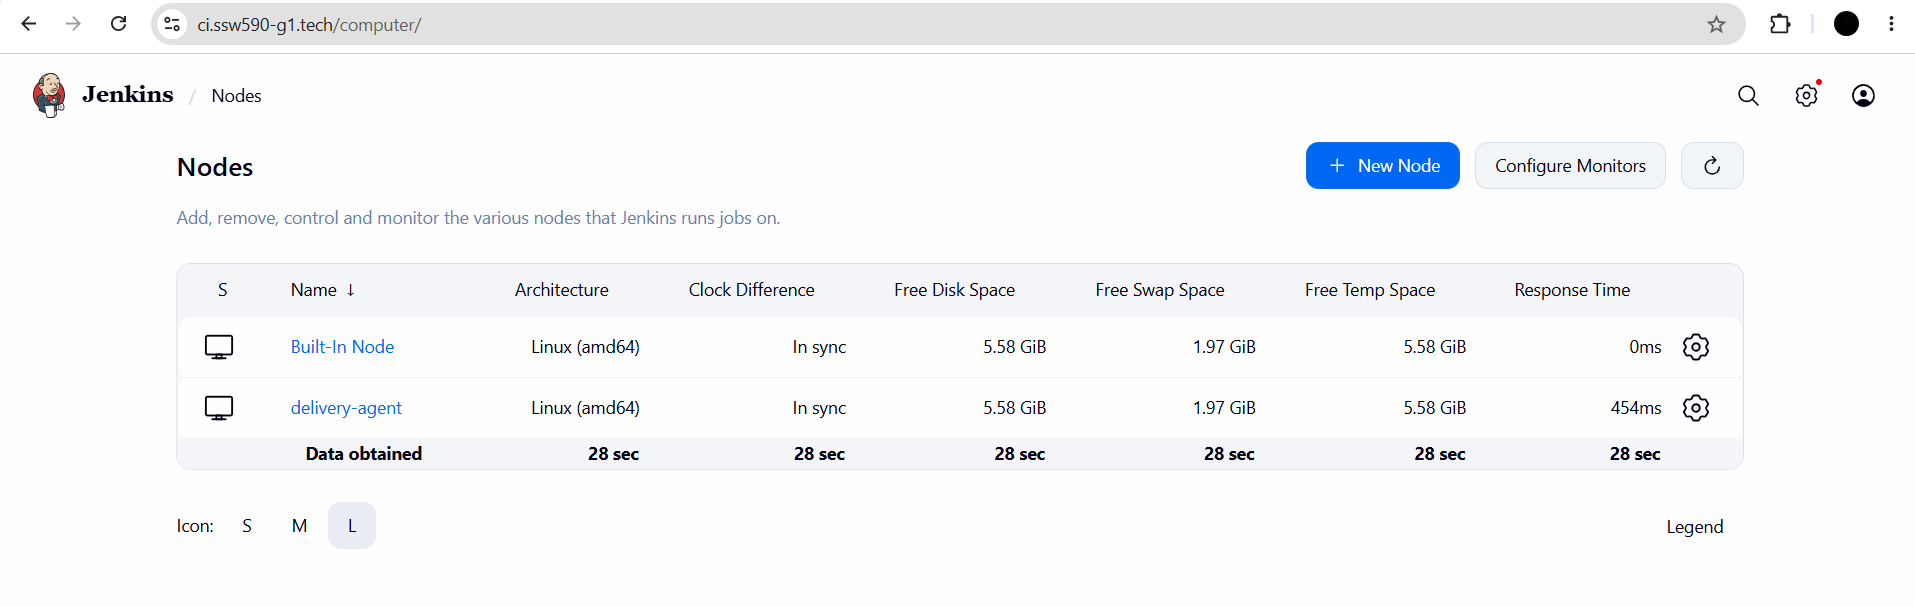
\includegraphics[width=0.9\linewidth]{evidence/206-jenkins-nodes-delivery-agent-linux-online-bd-2026-11-13.png}
\caption{Jenkins Nodes page: \texttt{delivery-agent} online as Linux (BD's screenshot).}
\label{Fig:E206}
\end{figure}

\begin{figure}[htbp]
\centering
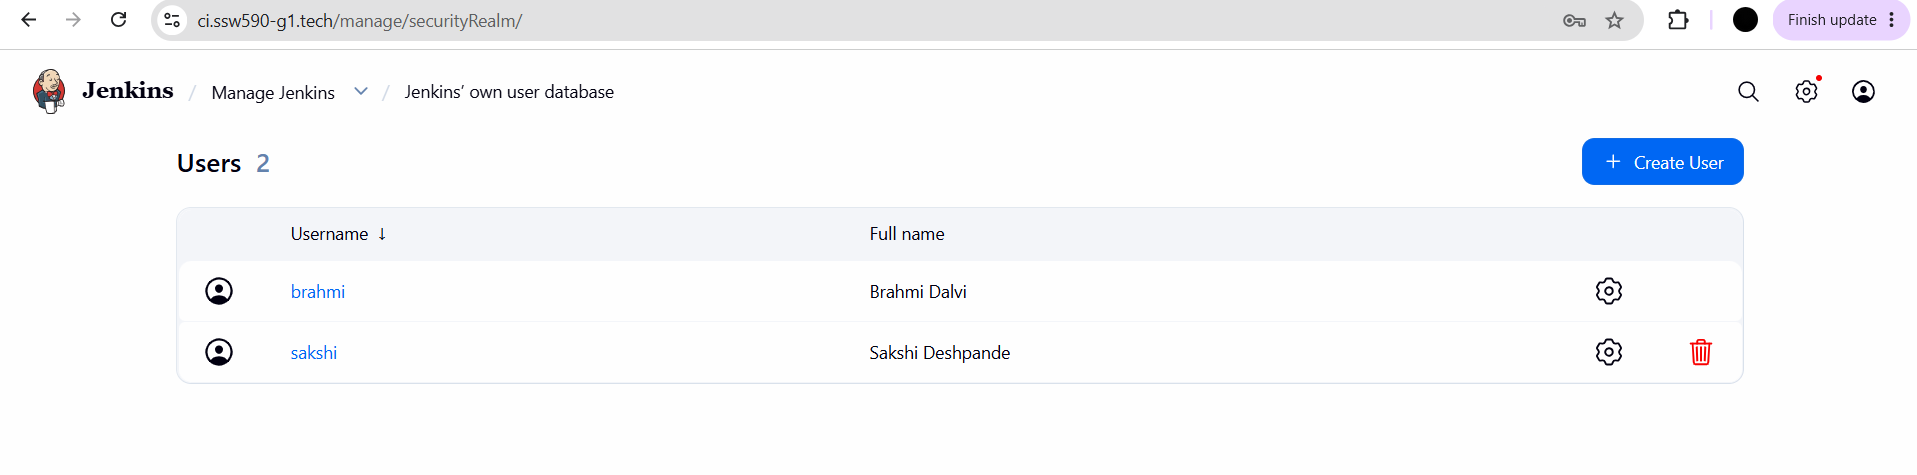
\includegraphics[width=0.9\linewidth]{evidence/210-jenkins-users-brahmi-sakshi-approver-ids-bd-2026-11-14.png}
\caption{The two Jenkins users, \texttt{brahmi} and \texttt{sakshi}, the only approvers (BD's screenshot).}
\label{Fig:E210}
\end{figure}

\begin{longlisting}
\inputminted[fontsize=\scriptsize]{text}{evidence/212-first-delivery-run-build-5-pip-audit-cache-failure-and-fix-bd-2026-11-16.txt}
\caption{Build \#5: the first delivery run failed on a root-owned cache directory, and the fix (real output).}
\label{Listing:E212}
\end{longlisting}

\begin{figure}[htbp]
\centering
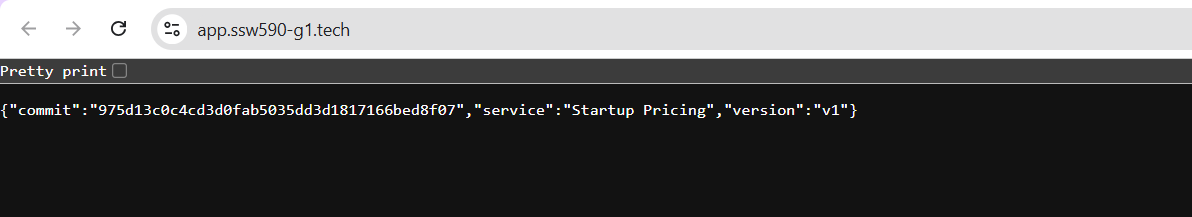
\includegraphics[width=0.9\linewidth]{evidence/218-app-ssw590-g1-tech-v1-in-browser-bd-2026-11-17.png}
\caption{The production URL in a browser after the first release (BD's screenshot).}
\label{Fig:E218}
\end{figure}

\begin{figure}[htbp]
\centering
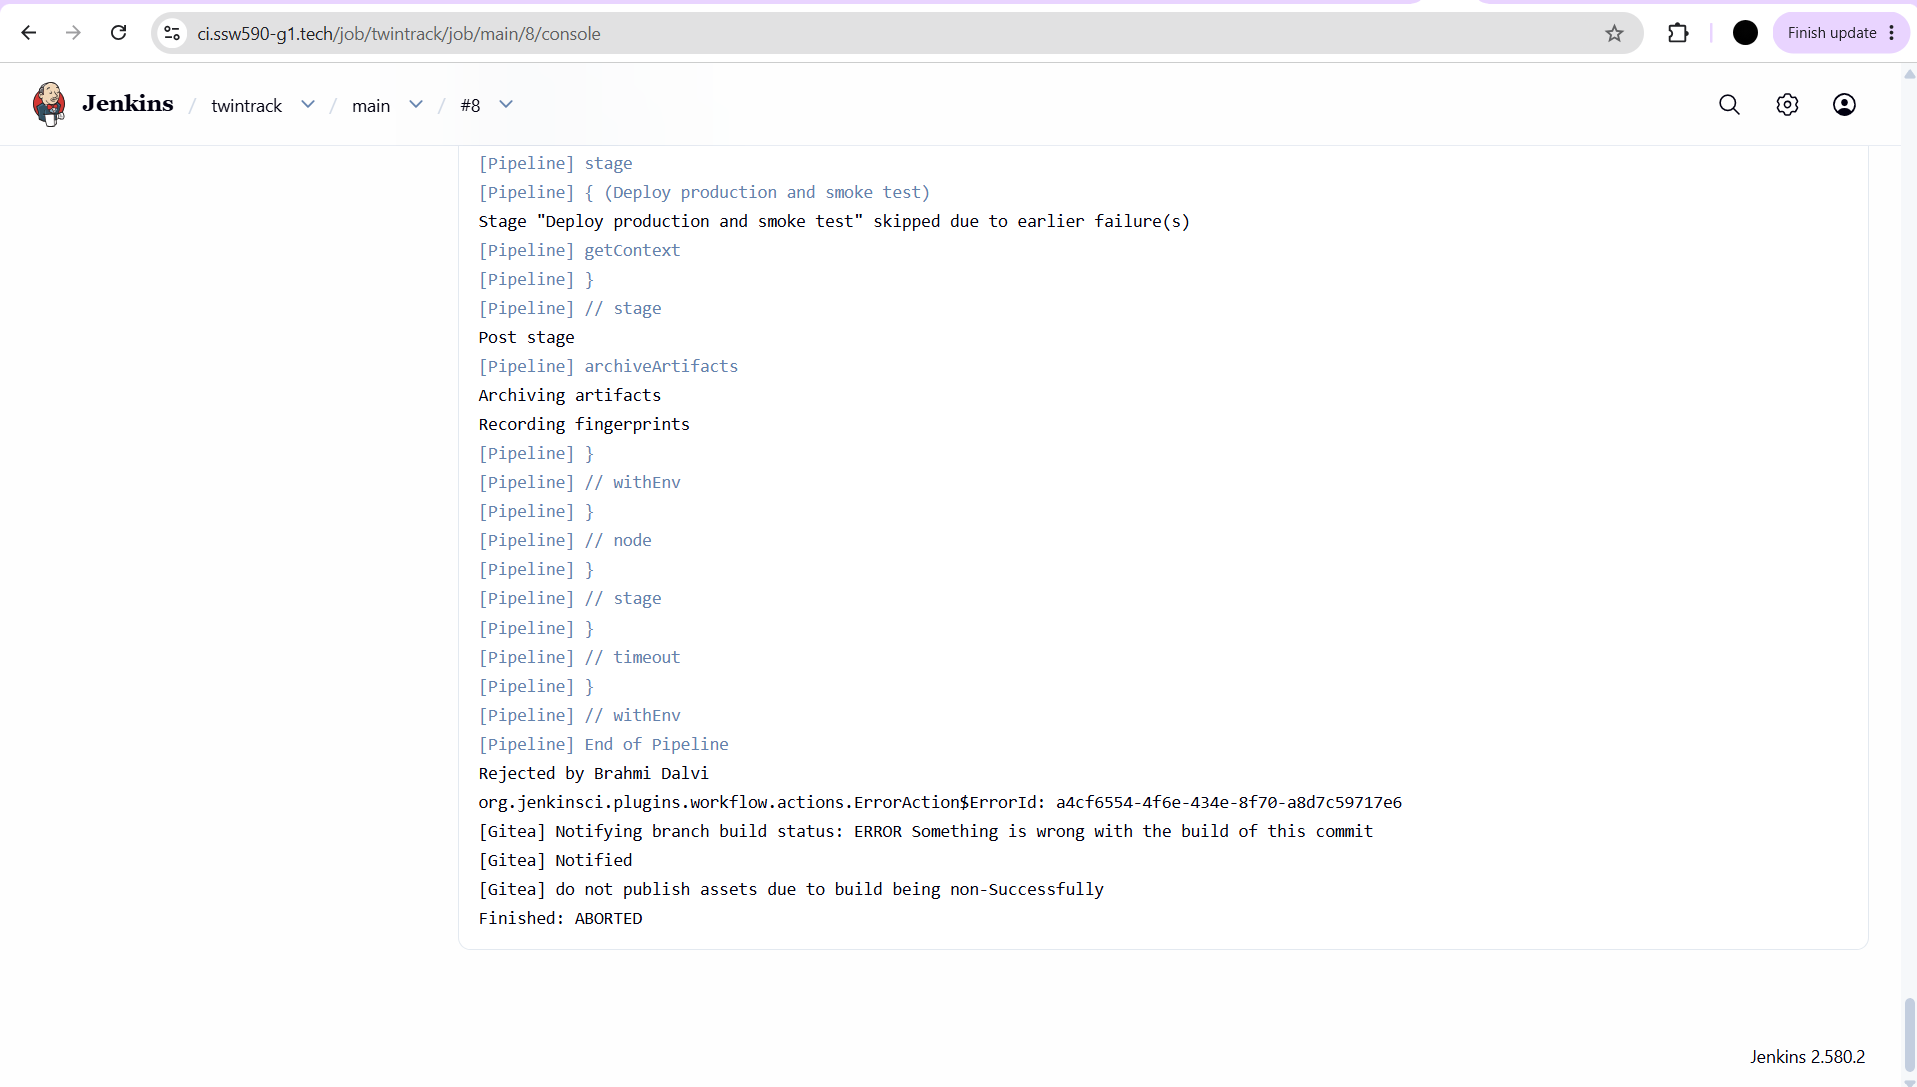
\includegraphics[width=0.9\linewidth]{evidence/221-build-8-aborted-rejected-by-brahmi-bd-2026-11-17.png}
\caption{Build \#8 ends \emph{Rejected by Brahmi Dalvi}: staged, not promoted (BD's screenshot).}
\label{Fig:E221}
\end{figure}

\begin{longlisting}
\inputminted[fontsize=\scriptsize]{text}{evidence/216-build-7-v1-released-staging-then-production-same-digest-bd-2026-11-17.txt}
\caption{Build \#7, November 17, 2026: v1 to staging, approval by \texttt{brahmi}, the same digest to production (real output).}
\label{Listing:E216}
\end{longlisting}

\begin{figure}[htbp]
\centering
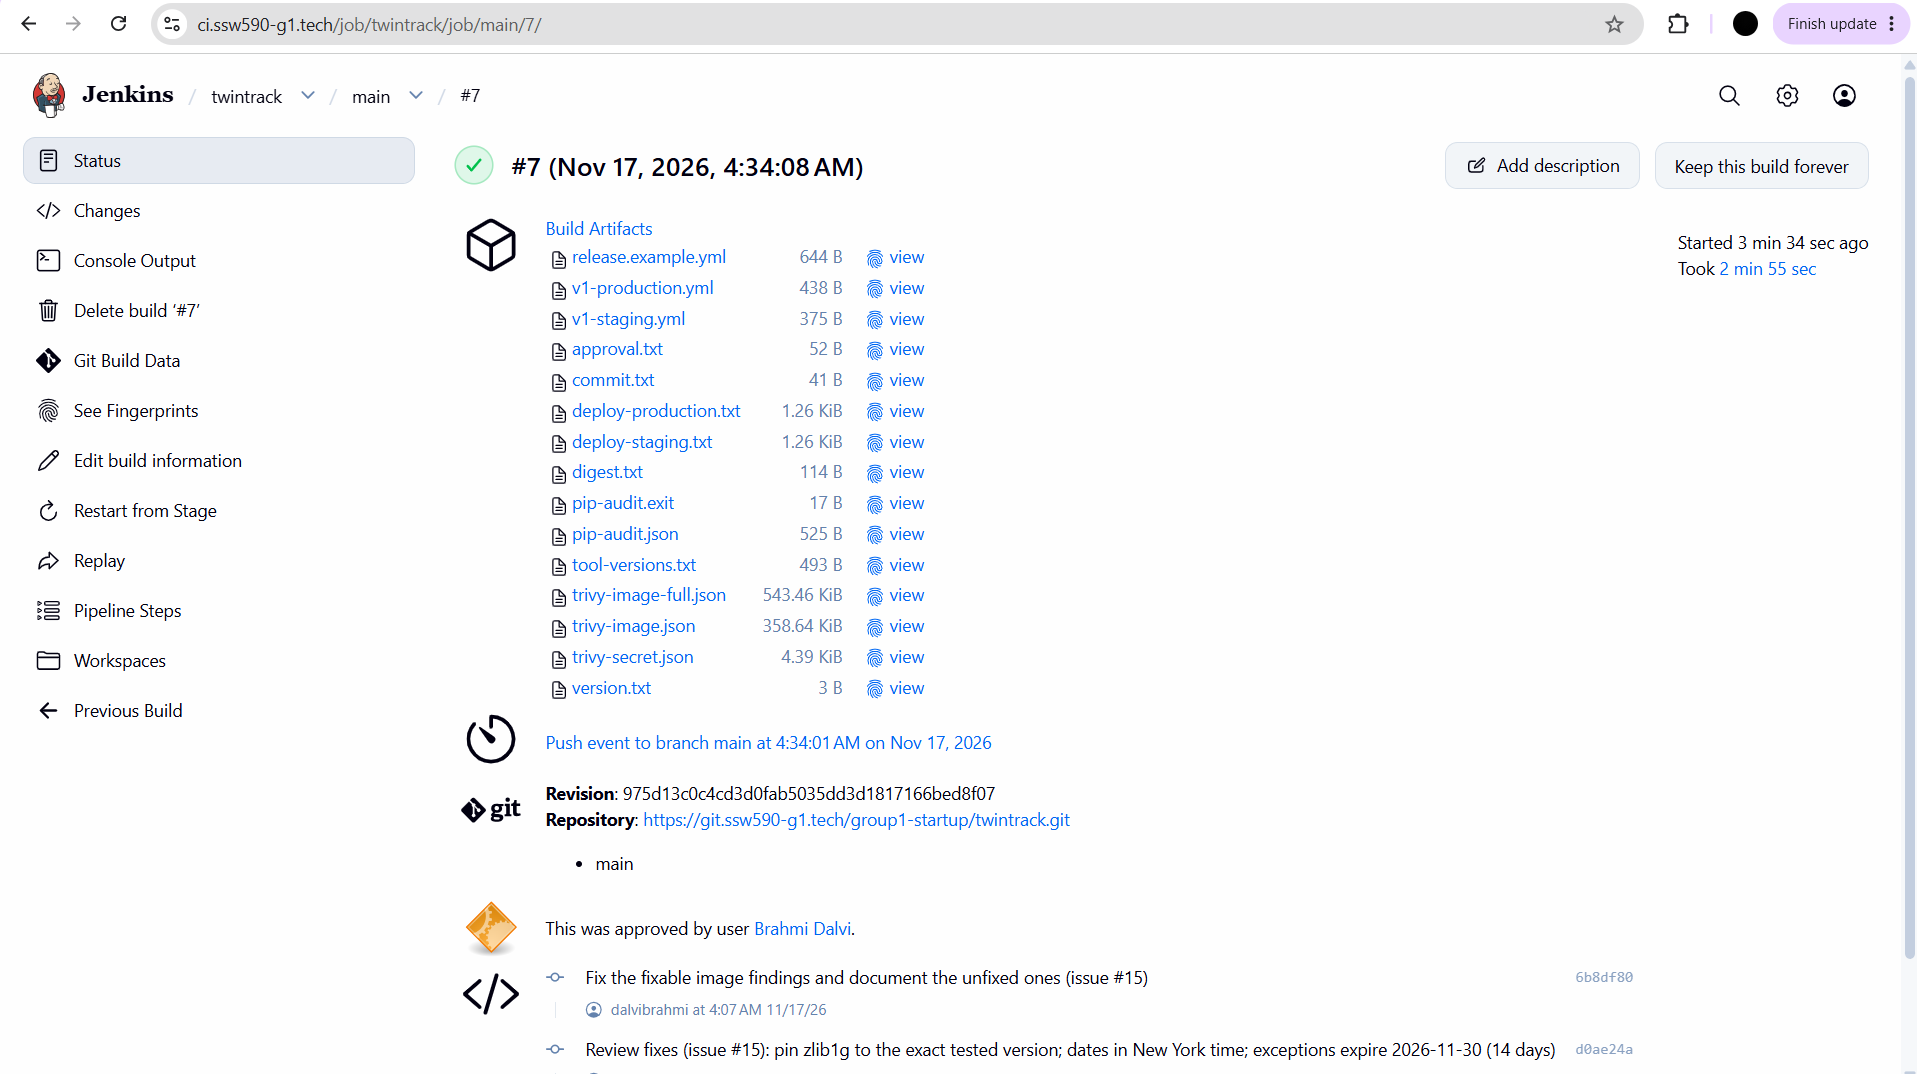
\includegraphics[width=0.9\linewidth]{evidence/217-build-7-success-artifacts-approved-by-brahmi-bd-2026-11-17.png}
\caption{Jenkins build \#7: success, 16 archived artifacts, ``approved by user Brahmi Dalvi'' (BD's screenshot).}
\label{Fig:E217}
\end{figure}

\begin{figure}[htbp]
\centering
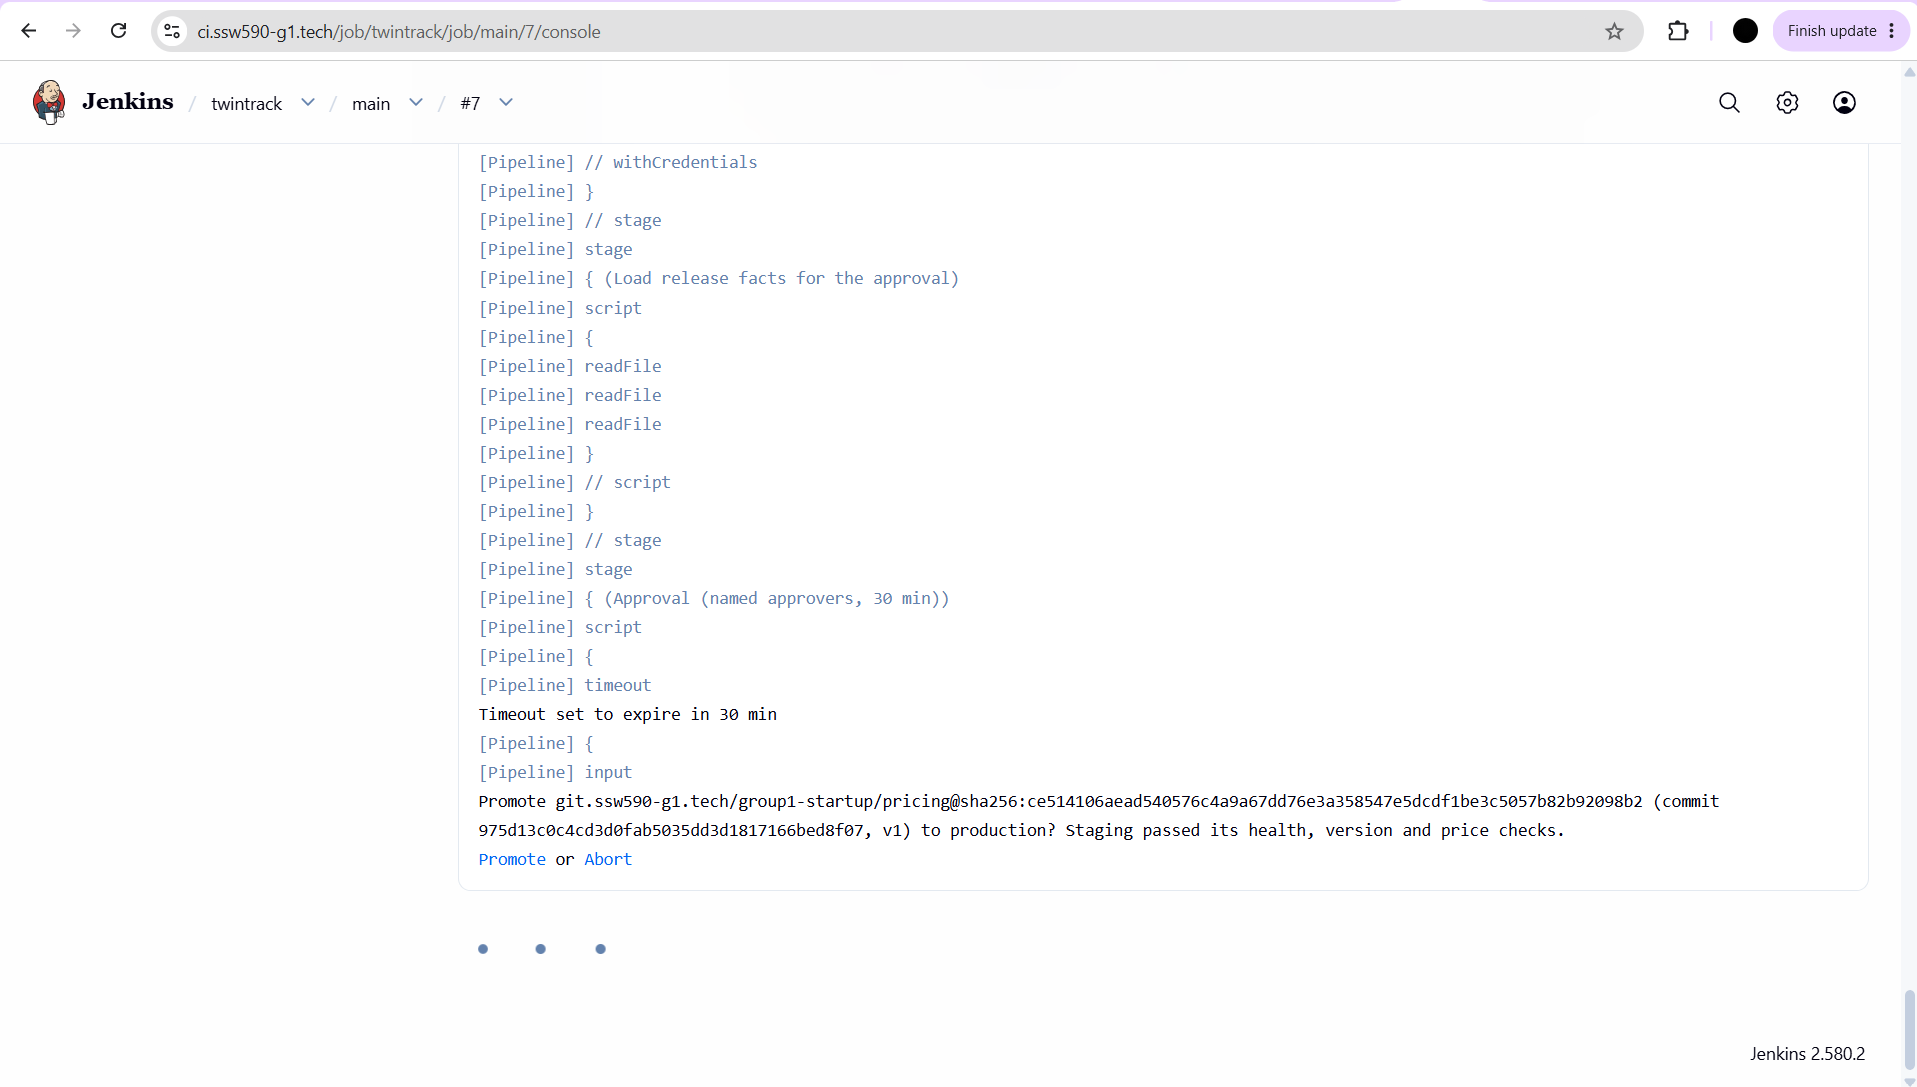
\includegraphics[width=0.9\linewidth]{evidence/214-build-7-approval-prompt-promote-or-abort-bd-2026-11-17.png}
\caption{The approval prompt of build \#7: digest, commit, version, Promote or Abort, 30-minute timeout (BD's screenshot).}
\label{Fig:E214}
\end{figure}

\begin{figure}[htbp]
\centering
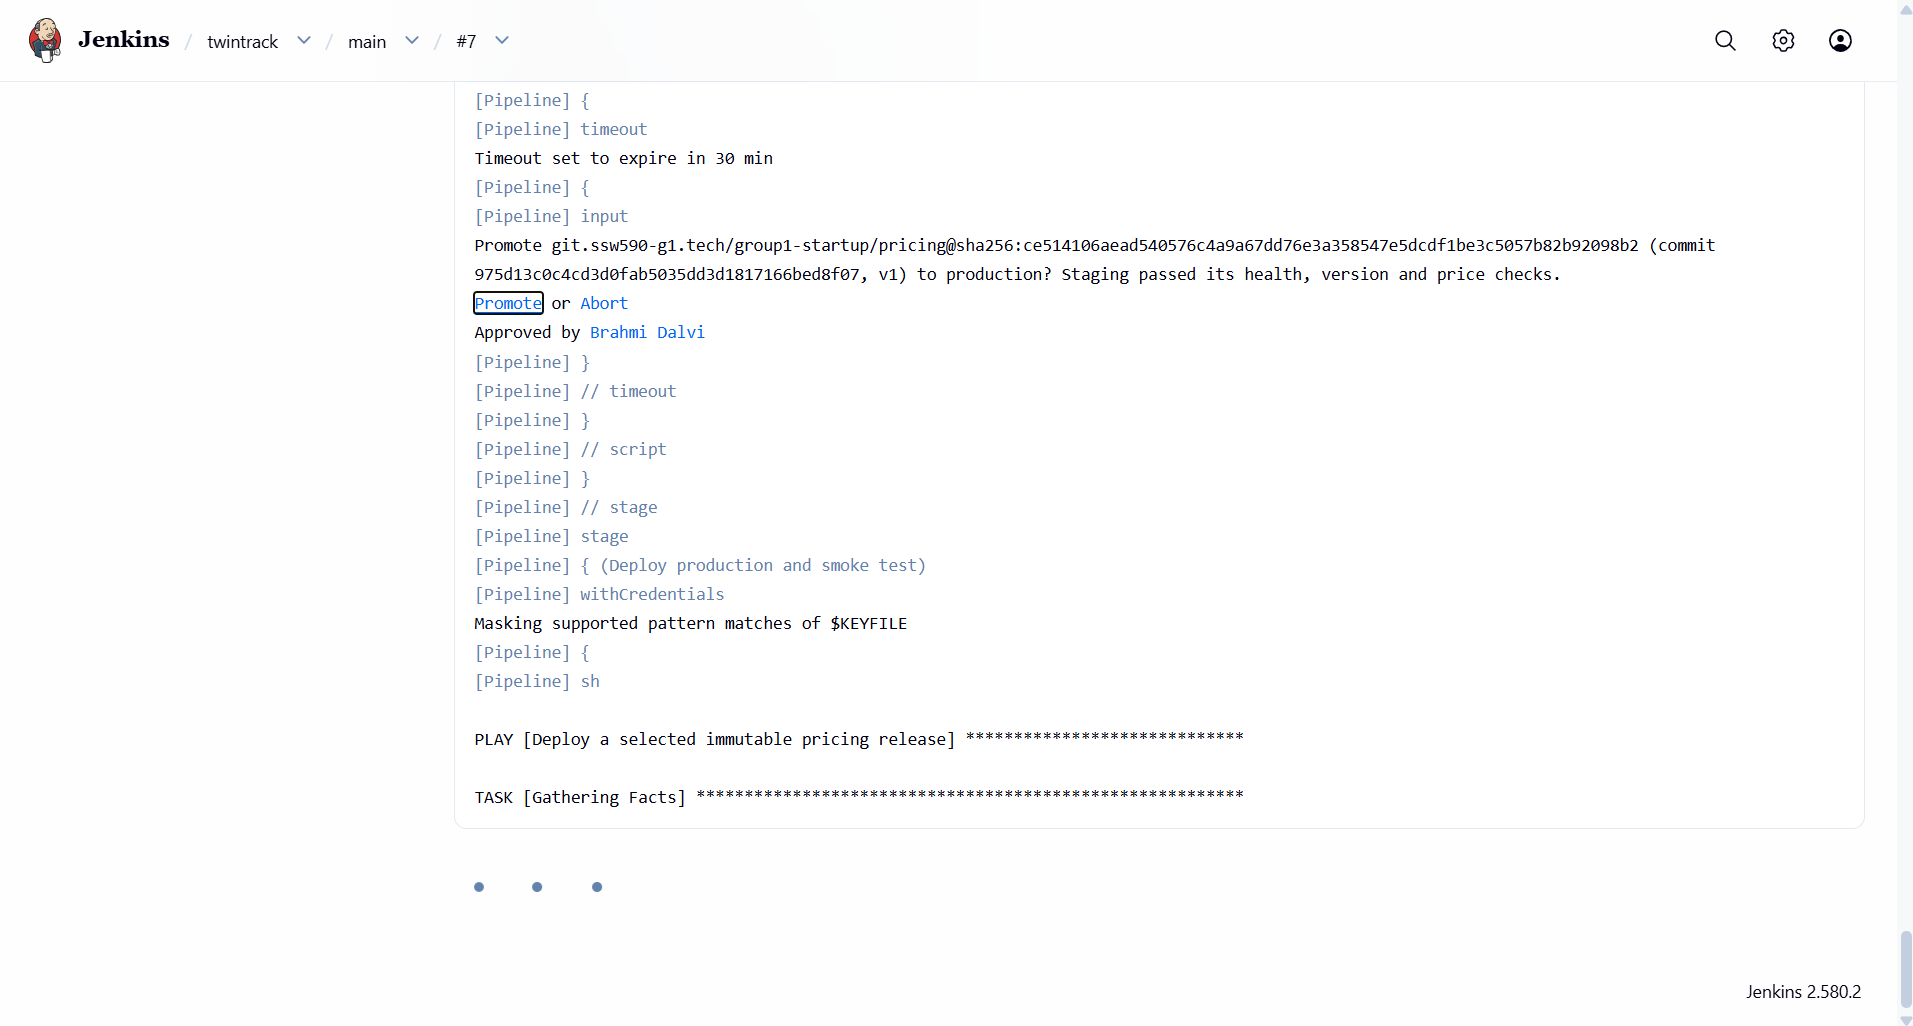
\includegraphics[width=0.9\linewidth]{evidence/215-build-7-approved-by-brahmi-production-deploy-started-bd-2026-11-17.png}
\caption{Build \#7 after the click: ``Approved by Brahmi Dalvi'', then the production deploy starts (BD's screenshot).}
\label{Fig:E215}
\end{figure}

\begin{longlisting}
\inputminted[fontsize=\scriptsize]{text}{evidence/230-build-11-v2-staging-verified-before-promotion-bd-2026-11-18.txt}
\caption{Build \#11 (v2) before promotion: scans, the staging record and public checks (real output).}
\label{Listing:E230}
\end{longlisting}

\begin{figure}[htbp]
\centering
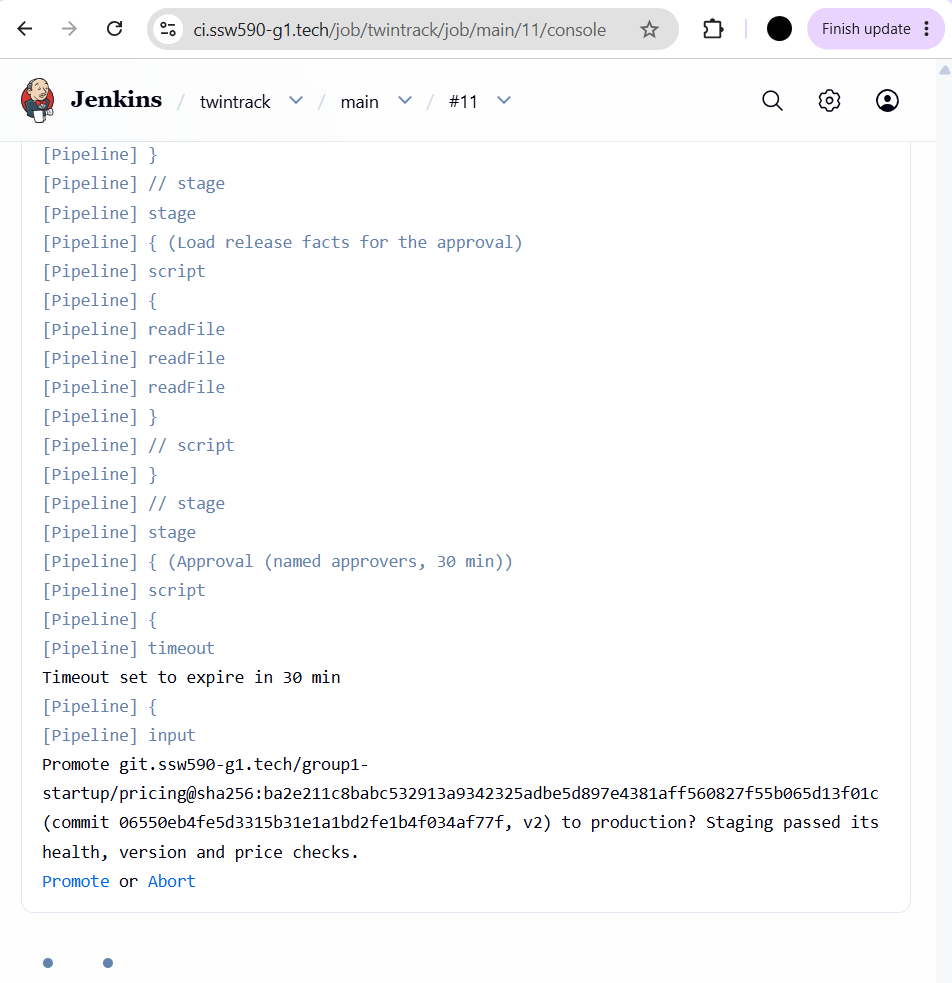
\includegraphics[width=0.9\linewidth]{evidence/229-build-11-v2-approval-prompt-bd-2026-11-18.png}
\caption{The approval prompt of build \#11 (v2) (BD's screenshot).}
\label{Fig:E229}
\end{figure}

\begin{longlisting}
\inputminted[fontsize=\scriptsize]{text}{evidence/231-build-11-v2-promoted-production-serves-v2-total-36-bd-2026-11-18.txt}
\caption{v2 promoted to production, November 17, 2026, 21:21~EST (real output).}
\label{Listing:E231}
\end{longlisting}

\begin{figure}[htbp]
\centering
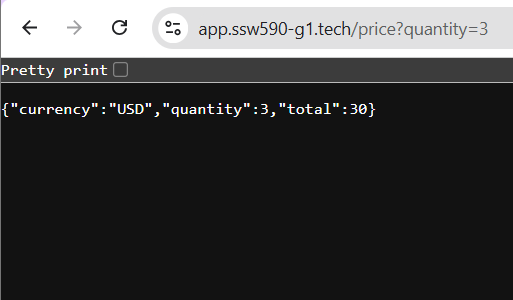
\includegraphics[width=0.9\linewidth]{evidence/235-app-price-quantity-3-total-30-after-rollback-in-browser-bd-2026-11-18.png}
\caption{Production after the v2 release: \texttt{/price?quantity=3} (BD's screenshot taken after the rollback of Section~\ref{Section:deliveryRecovery}).}
\label{Fig:E235}
\end{figure}

\begin{longlisting}
\inputminted[fontsize=\scriptsize]{text}{evidence/222-build-8-merge-of-pr-22-staged-not-promoted-aborted-bd-2026-11-17.txt}
\caption{Build \#8: staged, not promoted, aborted at the approval (real output).}
\label{Listing:E222}
\end{longlisting}

\begin{longlisting}
\inputminted[fontsize=\scriptsize]{text}{evidence/223-build-9-release-records-pr-19-delivery-skipped-by-changeset-bd-2026-11-17.txt}
\caption{Build \#9, the merge of the release-records pull request: the delivery stage is skipped (real output).}
\label{Listing:E223}
\end{longlisting}


% ===== BD region: row 5 (15 points) =====
\section{Security scans, policy and credentials (15 points)}\label{Section:deliveryScans}
\textbf{Owner:} BD. \textbf{Status:} policy written before the first release; one real block and one synthetic block recorded \StatusPass; the instructor's acceptance of the dated exceptions is requested.

\paragraph{Policy (written before the release).} The file \texttt{scan-policy.md} (course repository, \texttt{assignment-8/bd-work}) fixes what is scanned, when, and what blocks:
\begin{tabularx}{\linewidth}{L{3.2cm}L{3.2cm}Y}
\caption{Scan policy\label{Table:ScanPolicy}}\\
\toprule \textbf{What} & \textbf{Tool} & \textbf{When and what blocks}\\ \midrule
\endfirsthead
\toprule \textbf{What} & \textbf{Tool} & \textbf{When and what blocks}\\ \midrule
\endhead \bottomrule \endlastfoot
Python dependencies & pip-audit 2.10.1 on the hashed lock & before the build; any known vulnerability, a scanner error, or a missing report blocks.\\
Secrets in the source & Trivy 0.76.2, file-system secret scan & before the build; any finding blocks.\\
Image & Trivy image scan, HIGH and CRITICAL & after the build, before the push; any finding not covered by a dated exception blocks.\\
\end{tabularx}
Fixes come first. A finding with a fixed version is fixed (bump the dependency or the base, rebuild, rescan). An unfixed finding needs a written exception with the identifier, the reason, an owner and an expiry no later than 14 days,
reviewed in a pull request by the other person; an expired exception blocks again. There is no \texttt{|| true} anywhere in the pipeline.

\paragraph{The gate on the real release.} Build \#6 passed tests, pip-audit and the secret scan, built the image, and then the image scan stopped it: 53 HIGH findings and no CRITICAL, 47 of them without any fixed version (\ListRef{213}).
Nothing was pushed or deployed. Six findings had a fix and were fixed in the Dockerfile in pull request \#16 (the \texttt{zlib1g} security update, pinned to the exact version read from the tested image, and \texttt{pip}, \texttt{setuptools} and \texttt{wheel} removed
after the locked install, which also removed the vendored urllib3, msgpack and setuptools findings). The 47 rows are 11 CVE identifiers in Debian base-image packages (util-linux, acl, ncurses, sqlite, systemd and perl); each is listed in \texttt{.trivyignore.yaml}
with a reason in \texttt{security/exceptions.md}. The base-image findings are about local privilege escalation, mount helpers and libraries the service does not call; the service runs as UID 10001 on a read-only file system with all capabilities dropped.
\textbf{The exceptions expire on 2026-11-30 at 00:00~UTC, that is Sunday, November 29, 2026, 7~pm in New York}; after that every build blocks again until a reviewed pull request renews or removes them. The instructor's acceptance is requested for the use of these exceptions.

\paragraph{What reached the registry.} The package page of the \texttt{pricing} image listed three versions when the screenshot was taken on November 17, 2026: the commits \texttt{975d13c} (v1, build \#7), \texttt{102da1d} (build \#8, staged and not promoted) and \texttt{06550eb} (v2, build \#11); the two builds of the failed-deployment drill added \texttt{306242f} (the drill) and \texttt{99a061e} (the restore), so it holds five versions in the final state (\ListRef{243}, \ListRef{245}). The image of the blocked build \#6 and nothing of the fixture build \#12 was ever pushed, which is what the order scan, then push, guarantees The page of the v2 version shows the digest the pipeline recorded and the user \texttt{jenkins-bot} as publisher (\FigRef{242}).

\paragraph{After the fix.} Every later build keeps the full report (\texttt{trivy-image-full.json}: 47 HIGH rows) and gates on the filtered one (0 rows). The tested change: the image built from the modified Dockerfile scans with 0 findings and the service
answered \texttt{/health} and \texttt{/price}; the pinned package installed in the real build (\ListRef{213}, \ListRef{216}).

\paragraph{Blocked fixture.} To show each scanner block a bad change without putting anything into the repository, BD replayed build \#11 with a fixture step: a temporary directory with a known-vulnerable pin (urllib3 1.25.8) and a fake credential in the shape of a GitHub token
(assembled at run time, never valid). Result (\ListRef{239}): pip-audit exit 1 with 21 vulnerabilities, Trivy secret scan exit 1 with one CRITICAL finding of rule \texttt{github-pat}, the line \texttt{BLOCKED}, and every later stage (image build, push, staging, approval, production)
skipped; no image was built, nothing was pushed, both environments were untouched, and the temporary directory was removed.

\paragraph{Credentials and access.} Nothing secret is in Git, in the chat with the assistant, in command arguments, or in logs; BD typed or pasted each secret herself.
\begin{tabularx}{\linewidth}{L{3.2cm}L{3.4cm}Y}
\caption{Credentials of the delivery pipeline\label{Table:DeliveryCredentials}}\\
\toprule \textbf{Credential} & \textbf{Where it lives} & \textbf{Scope and risk}\\ \midrule
\endfirsthead
\toprule \textbf{Credential} & \textbf{Where it lives} & \textbf{Scope and risk}\\ \midrule
\endhead \bottomrule \endlastfoot
\texttt{deploy-ssh-key} & Jenkins credential only (\FigRef{204}); the local key files were deleted & ed25519 key for the \texttt{deploy} account: key-only login, no password, passwordless \texttt{sudo} (documented as host-administrator power, \ListRef{203}); revoke by deleting the line in \texttt{authorized\_keys}.\\
\texttt{gitea-registry-\allowbreak write} & Jenkins credential, bound only in the push stage & Gitea user \texttt{jenkins-bot}, package scope only, with an expiry (\FigRef{207}); the account has more rights in the \texttt{developers} team (\FigRef{209}), so the token is narrower than the account.\\
registry read token & root's \texttt{/root/.docker/\allowbreak config.json} on the host & read-only, with an expiry; stored in plain text, readable by root and so by the \texttt{deploy} account and the agent; used for the pull by digest (\ListRef{211}).\\
Jenkins users & Jenkins' own database & exactly \texttt{brahmi} and \texttt{sakshi} may approve (\FigRef{210}).\\
\end{tabularx}
The deploy path is the host's Docker bridge (alias \texttt{deploy-target}) with a pinned SSH host key, because the host cannot reach its own Elastic IP on port 22 through the security group (\ListRef{201}). The two public hostnames, \texttt{staging} and \texttt{app}, are served by Caddy with
Let's Encrypt certificates issued within seconds of the reload (\ListRef{208}); both are public on purpose because the service is stateless and Ansible checks the public name.

\begin{longlisting}
\inputminted[fontsize=\scriptsize]{text}{evidence/213-build-6-image-scan-gate-blocked-the-release-bd-2026-11-16.txt}
\caption{Build \#6, November 16, 2026: the image scan blocked the release (real output).}
\label{Listing:E213}
\end{longlisting}

\begin{longlisting}
\inputminted[fontsize=\scriptsize]{text}{evidence/239-blocked-fixture-secret-and-vulnerable-dependency-bd-2026-11-18.txt}
\caption{Blocked fixture: pip-audit and the secret scan stop a replayed build (real output).}
\label{Listing:E239}
\end{longlisting}

\begin{longlisting}
\inputminted[fontsize=\scriptsize]{text}{evidence/201-ssh-reachability-from-host-and-containers-to-own-public-and-private-address-bd-2026-11-12.txt}
\caption{SSH from the host and from containers to its own public and private address (real output).}
\label{Listing:E201}
\end{longlisting}

\begin{longlisting}
\inputminted[fontsize=\scriptsize]{text}{evidence/208-caddy-blocks-staging-and-app-applied-certificates-issued-bd-2026-11-14.txt}
\caption{The two Caddy blocks for staging and app; the certificates are issued (real output).}
\label{Listing:E208}
\end{longlisting}

\begin{longlisting}
\inputminted[fontsize=\scriptsize]{text}{evidence/203-deploy-account-created-key-only-sudo-bd-2026-11-12.txt}
\caption{The deploy account (real output pasted by BD).}
\label{Listing:E203}
\end{longlisting}

\begin{figure}[htbp]
\centering
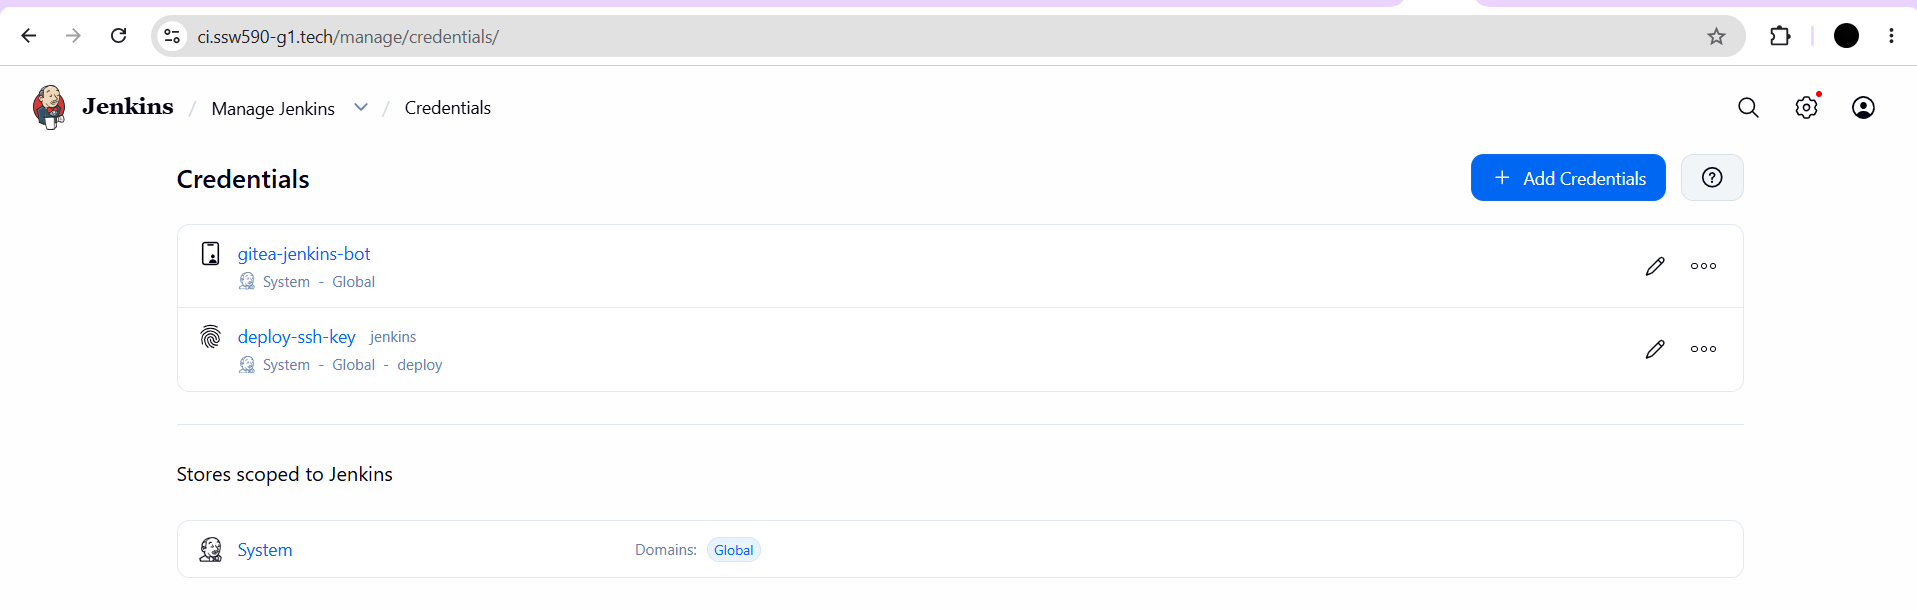
\includegraphics[width=0.9\linewidth]{evidence/204-jenkins-credentials-list-deploy-ssh-key-added-bd-2026-11-12.png}
\caption{Jenkins credentials after the deploy key was added (BD's screenshot).}
\label{Fig:E204}
\end{figure}

\begin{figure}[htbp]
\centering
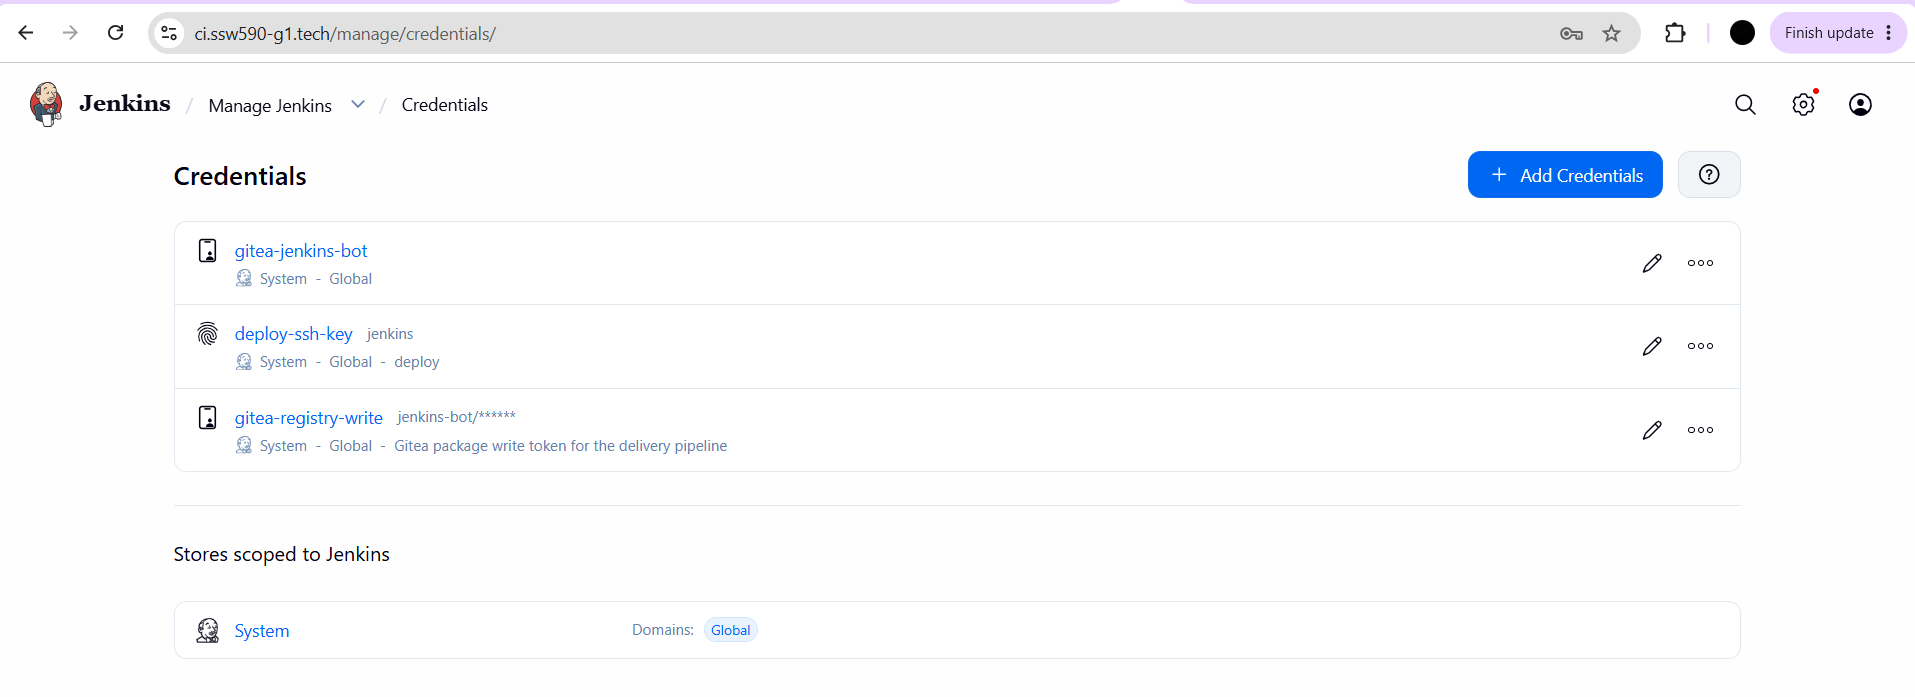
\includegraphics[width=0.9\linewidth]{evidence/207-jenkins-credentials-gitea-registry-write-added-bd-2026-11-14.png}
\caption{Jenkins credentials after the registry write credential was added; the token is masked (BD's screenshot).}
\label{Fig:E207}
\end{figure}

\begin{figure}[htbp]
\centering
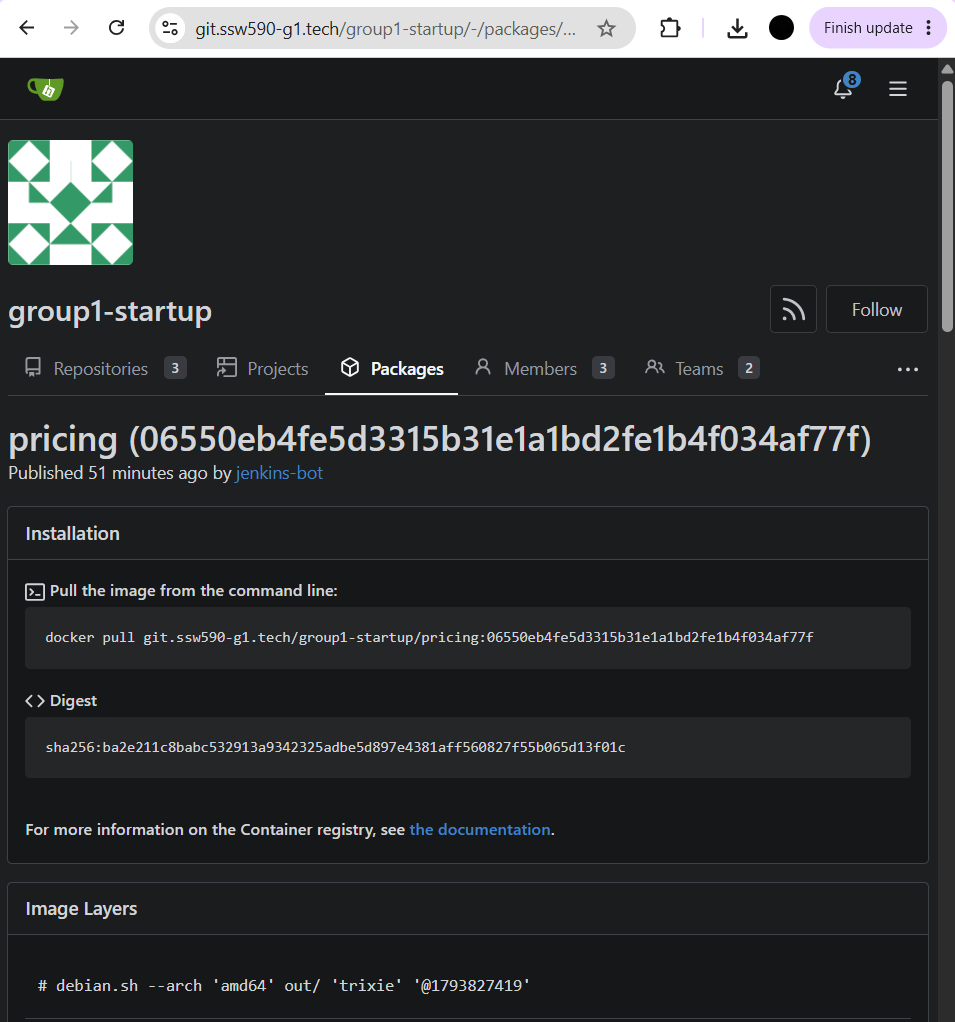
\includegraphics[width=0.9\linewidth]{evidence/242-gitea-package-pricing-v2-published-by-jenkins-bot-digest-bd-2026-11-18.png}
\caption{The package page of the v2 image: published by \texttt{jenkins-bot}, digest \texttt{sha256:ba2e211c\ldots f01c} (BD's screenshot).}
\label{Fig:E242}
\end{figure}

\begin{figure}[htbp]
\centering
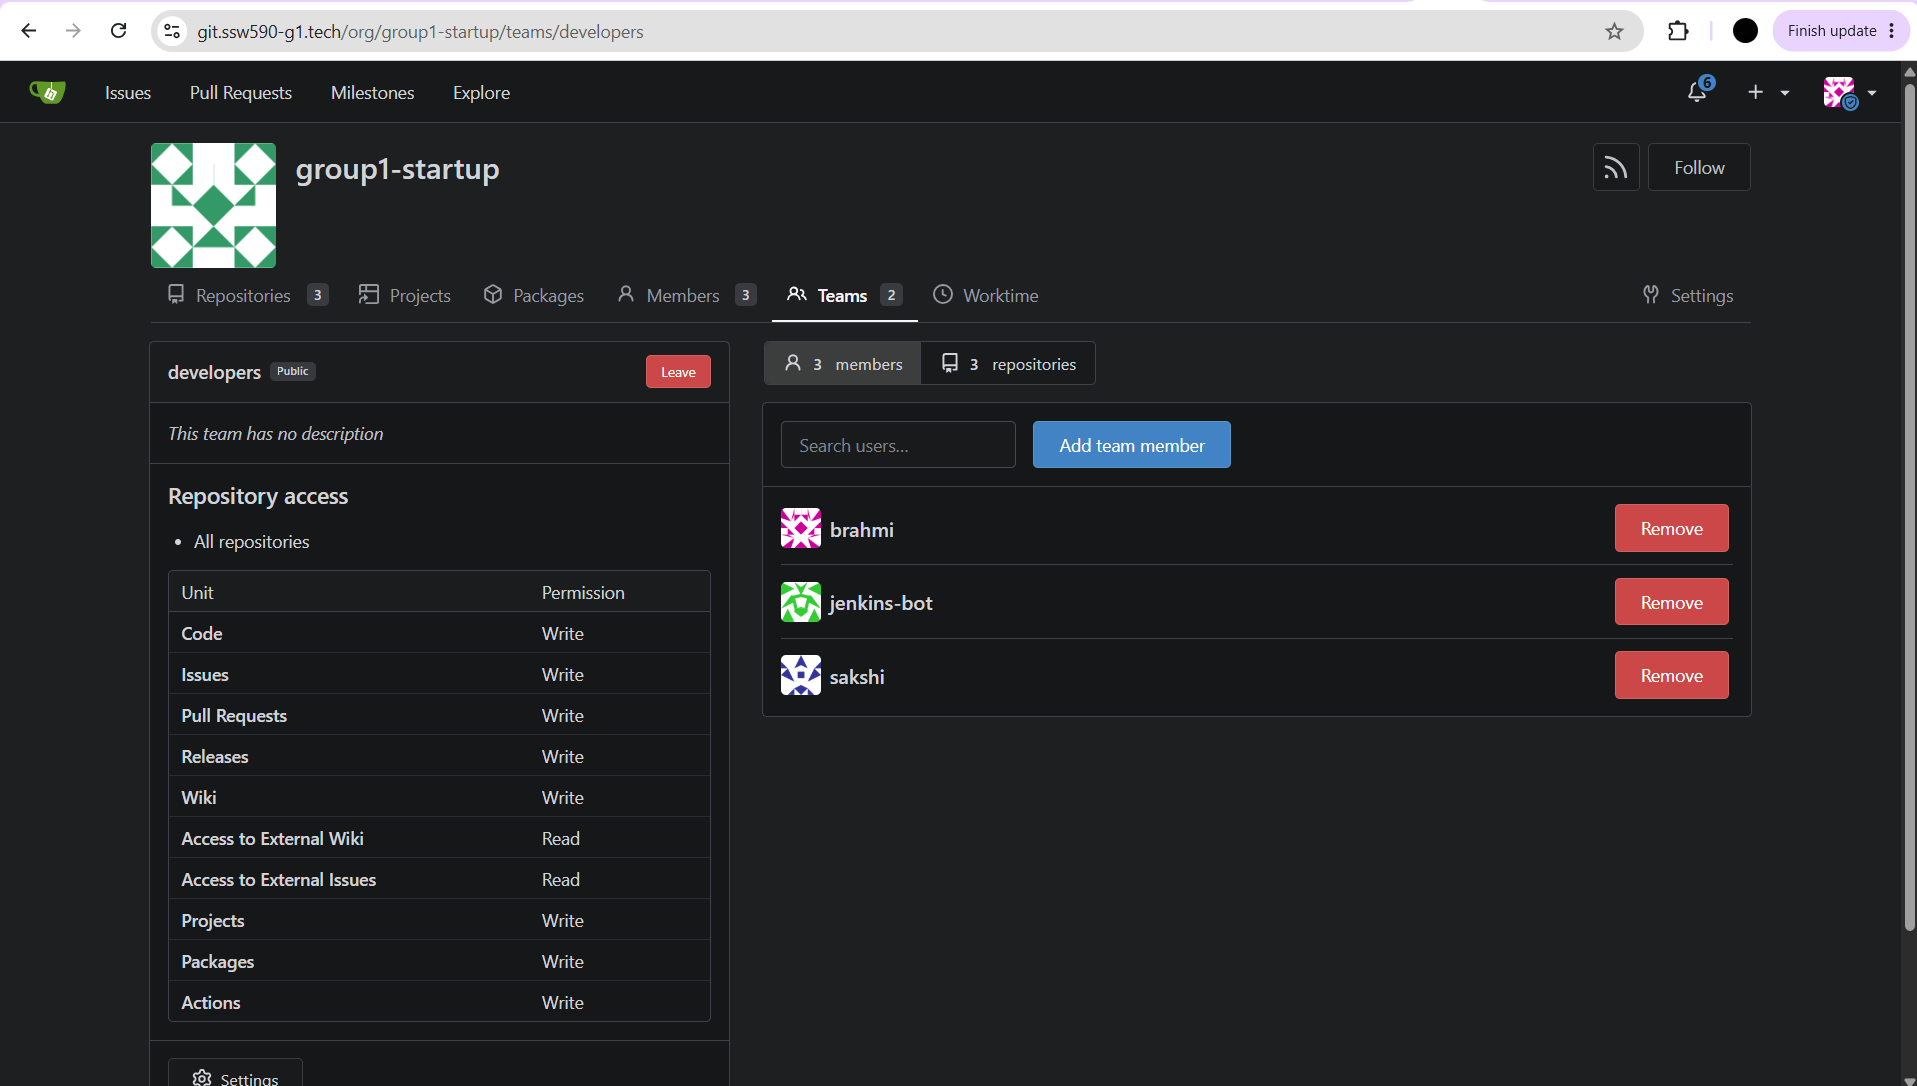
\includegraphics[width=0.9\linewidth]{evidence/209-gitea-developers-team-jenkins-bot-packages-write-bd-2026-11-14.png}
\caption{The \texttt{developers} team: \texttt{jenkins-bot} has Packages write (BD's screenshot).}
\label{Fig:E209}
\end{figure}

\begin{longlisting}
\inputminted[fontsize=\scriptsize]{text}{evidence/211-registry-read-login-root-and-pre-merge-check-bd-2026-11-16.txt}
\caption{Root's registry login and the pre-merge check (real output pasted by BD).}
\label{Listing:E211}
\end{longlisting}


% ===== BD region: row 6 (15 points) =====
\section{Rollback and staging recovery (15 points)}\label{Section:deliveryRecovery}
\textbf{Owner:} BD. \textbf{Status:} both recoveries run on November 17, 2026 (New York) \StatusPass.

\paragraph{The mechanism.} Both recoveries re-apply a \emph{release record} (exact digest, commit, expected version and total, public URL, network) with the same Ansible playbook as a normal release; nothing is rebuilt and no tag such as \texttt{latest} is used.
A second Jenkins job, \texttt{rollback} (file \texttt{Jenkinsfile.rollback}), accepts only \texttt{releases/v<n>-staging.yml} or \texttt{-production.yml}, checks that the record is tracked in \texttt{main}, that its \texttt{target\_env} agrees with the name, that the image is a digest, that the commit is 40 hexadecimal
characters and an ancestor of \texttt{main}, so a rollback cannot target an unreviewed release; a production record needs the same named approval, a staging record does not.
The v1 records are committed in \texttt{main} (pull request \#19, byte-identical to the archived artifacts of build \#7).

\paragraph{Three problems before it ran.} Builds \#1 to \#4 of the job failed without touching any server: the file was not on \texttt{main} yet; then Jenkins refused the whole file because of an invalid Groovy escape (a backslash-dot in a regular expression inside a triple-quoted
shell block): ``unexpected char: \textbackslash{}'' (\FigRef{224}, \ListRef{225}). BD's local checks missed it because they tested the unescaped shell text; a check script that finds invalid escapes was added, and the fix went through its own pull request (\#24), which BD merged as administrator without a review by SD because it was a one-line repair of a job that could not run. The first run of the fixed file stopped
at an unset parameter, which is the safe behaviour of \texttt{set -u}, and registered the parameter.

\paragraph{Unchanged second run (row 3).} With \texttt{releases/v1-staging.yml}: the first run changed 2 tasks (staging moved back from a staged candidate to the build \#7 digest), the second run of the same record showed \texttt{changed=0} and the container was not restarted; the production record, approved by BD, also showed \texttt{changed=0}
(\ListRef{228}).

\paragraph{Case A: production rollback v2 to v1 (job \texttt{rollback}, build \#8).} Trigger: v2 live in production. BD chose the record \texttt{releases/v1-production.yml}; the prompt named the digest \texttt{sha256:ce514106\ldots 98b2} (\FigRef{226}); BD approved at 02:23:37~UTC on November 18 (\FigRef{227});
Ansible ended \texttt{ok=9 changed=2 failed=0} and its smoke test asserted version v1, the right commit and total 30. The container started 12~seconds after the approval; public checks: version v1, commit \texttt{975d13c}, total 30 (\FigRef{234}, \FigRef{235}, \ListRef{232}).
A read-only observer on the server asked the production URL once a second (\ListRef{233}): the last v2 answer at 02:23:48, one 502 sample at 02:23:50, the first v1 answer at 02:23:51, that is about 2 to 3~seconds without a good answer, and the only non-200 line. The matching configuration came back with it: the rendered Compose file names the v1 digest again.

\paragraph{Case B, first drill: a missing image.} The failure was injected on purpose and traceably by replaying rollback build \#6 (the replay is build \#9 of the job) with the digest replaced by 64 zeros, an image that does not exist (the deploy key lives only in Jenkins and the job refuses records that are not in \texttt{main}, so a replay is the safe way).
Ansible failed at \emph{Converge application without rebuilding} with ``manifest unknown'', recap \texttt{ok=4 changed=1 failed=1} (\ListRef{237}). Compose pulls the image before it touches the running container, so staging stayed on the v2 container, healthy, still answering v2 and 36; only the rendered Compose file had changed to name the missing digest, a drift between configuration and running release.
Production was untouched and the approval and production stages are never reached after a failed staging deploy. Recovery: the same job as a normal run (build \#10) with \texttt{releases/v1-staging.yml}, \texttt{ok=9 changed=2 failed=0} (the Compose file restored, staging moved onto the known-good digest), verified at 02:46~UTC: version v1, commit \texttt{975d13c}, total 30 on both URLs (\ListRef{238}).
About 6~minutes passed between the failure and the verified recovery, most of it waiting for the person to start the second run. Staging ends on v1, the last release whose record is in \texttt{main}; to put v2 back, its record is committed in a reviewed pull request first.

\paragraph{Case B as the course describes it: a configuration commit.} The course asks for a separate configuration commit that binds Gunicorn to port 8001 in staging while the image's healthcheck still probes 8000, so BD did that too. Issue \#27 and pull request \#28 (merged by BD as administrator, a deliberate drill commit) changed three lines of \texttt{ansible/templates/compose.yaml.j2}: for staging only, the Compose command became \texttt{["gunicorn", "--bind", "0.0.0.0:8001", "app:app"]}. Jenkins built the merge commit \texttt{306242f} (tests, scans, image and push passed), and then \emph{Deploy staging} failed with \texttt{container pricing-staging-app-1 is unhealthy}, recap \texttt{ok=4 changed=1 failed=1} (\ListRef{243}). The run stopped there: no approval prompt, no production stage, production unchanged. Unlike the first drill, the image exists, so Compose replaced the running container with one that listens on 8001; staging answered 502 until the configuration was restored, about 12~minutes of planned outage, while production kept serving v1.

Recovery: the previous reviewed template was put back in its own pull request (\#29, merge \texttt{99a061e}; issue \#27 closed). The restore build (\#15) staged the restored configuration with \texttt{ok=9 changed=2 failed=0}, staging was healthy on port 8000 again and answered v2 with total 36, and BD aborted the build at the approval (\FigRef{244}, \ListRef{245}). Last, the \texttt{rollback} job re-applied the previous staging release record, \texttt{releases/v1-staging.yml}, on the restored \texttt{main}: \texttt{ok=9 changed=2 failed=0}, staging on the known-good digest \texttt{ce514106}\ldots, version v1 and total 30, production untouched (\ListRef{246}). The failure and the restore both stay in the history; the configuration commit and the release record were restored together, as the course requires.

\paragraph{What is not claimed.} The rollback was practised on a release whose previous version is still in the registry; if a registry image were deleted, a rollback to it would fail like the first drill of Case B. The runs were short because the service is a single stateless container; a service with data would need a data plan that this exercise does not cover.

\begin{longlisting}
\inputminted[fontsize=\scriptsize]{text}{evidence/228-restore-runs-staging-twice-and-production-changed-0-bd-2026-11-18.txt}
\caption{The three restore runs: staging record twice, then the production record (real output).}
\label{Listing:E228}
\end{longlisting}

\begin{figure}[htbp]
\centering
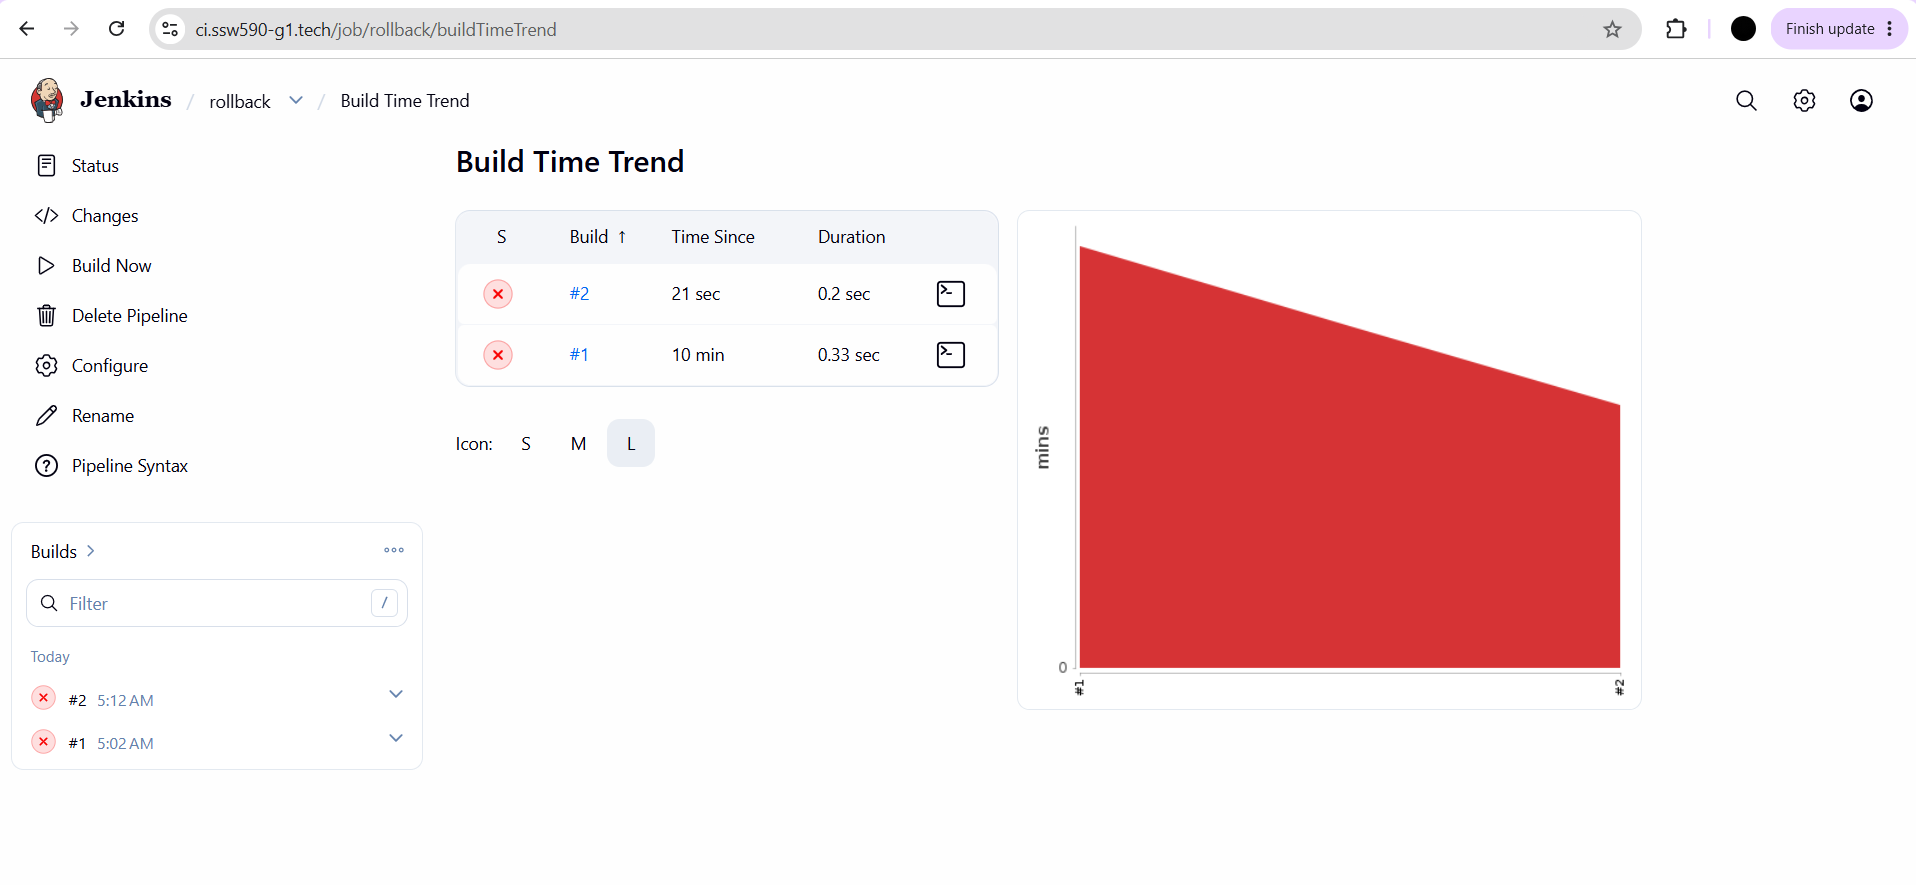
\includegraphics[width=0.9\linewidth]{evidence/224-rollback-job-builds-1-2-failed-groovy-escape-bd-2026-11-17.png}
\caption{The \texttt{rollback} job's first builds failed in under a second (BD's screenshot).}
\label{Fig:E224}
\end{figure}

\begin{longlisting}
\inputminted[fontsize=\scriptsize]{text}{evidence/225-rollback-job-first-runs-failed-groovy-escape-found-and-fixed-bd-2026-11-17.txt}
\caption{Why the first builds failed: an invalid Groovy escape, and the new check (real output).}
\label{Listing:E225}
\end{longlisting}

\begin{figure}[htbp]
\centering
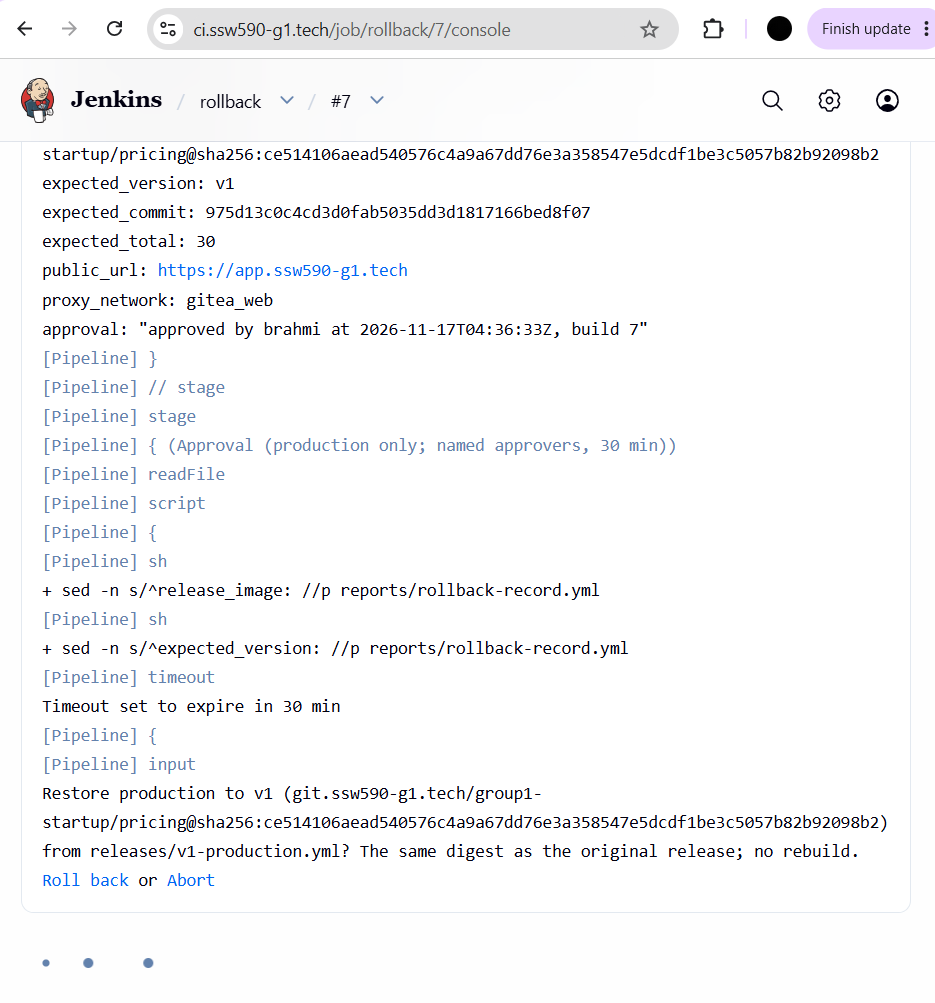
\includegraphics[width=0.9\linewidth]{evidence/226-rollback-job-build-7-approval-prompt-restore-production-v1-bd-2026-11-18.png}
\caption{The approval of the production rollback: the digest of v1, no rebuild (BD's screenshot).}
\label{Fig:E226}
\end{figure}

\begin{figure}[htbp]
\centering
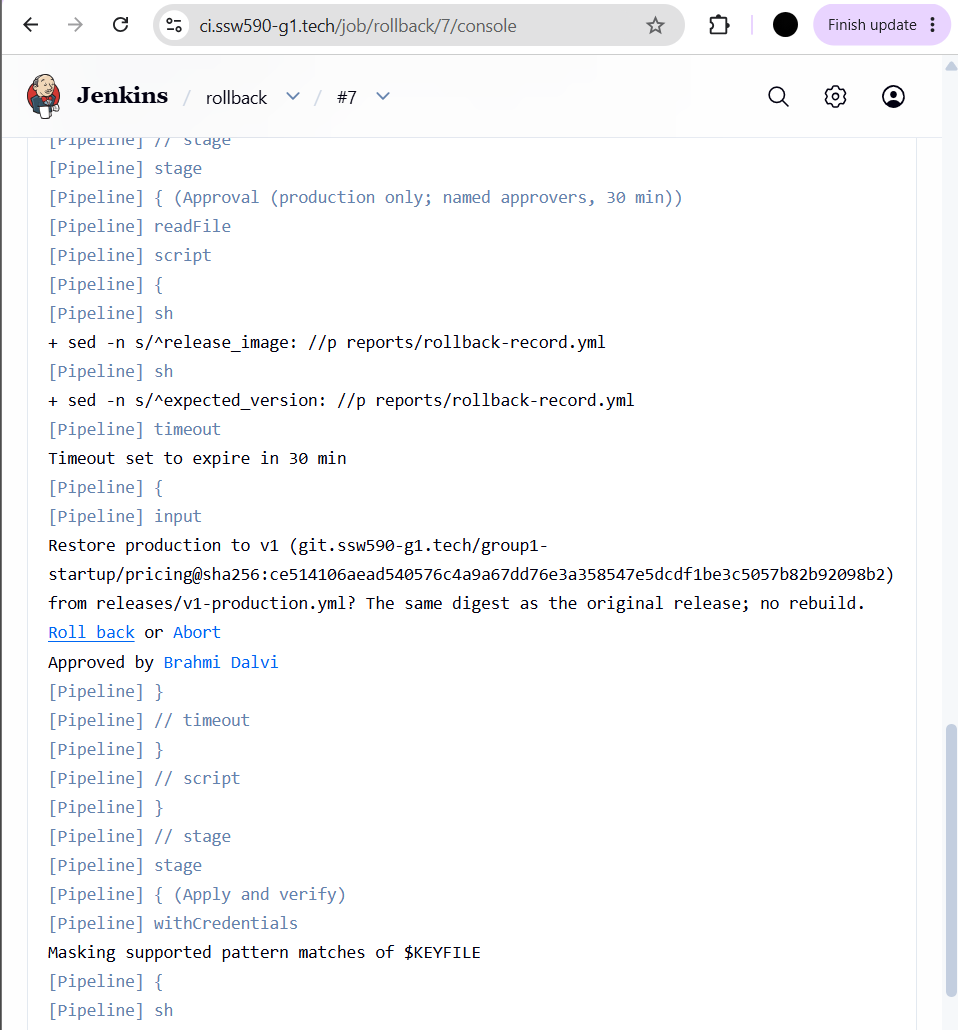
\includegraphics[width=0.9\linewidth]{evidence/227-rollback-job-build-7-approved-by-brahmi-apply-started-bd-2026-11-18.png}
\caption{After the click: ``Approved by Brahmi Dalvi'', Apply and verify starts (BD's screenshot).}
\label{Fig:E227}
\end{figure}

\begin{longlisting}
\inputminted[fontsize=\scriptsize]{text}{evidence/232-production-rollback-v2-to-v1-job-rollback-build-8-bd-2026-11-18.txt}
\caption{The production rollback v2 to v1: record, approval, Ansible, public checks (real output).}
\label{Listing:E232}
\end{longlisting}

\begin{longlisting}
\inputminted[fontsize=\scriptsize,firstline=50,lastline=62]{text}{evidence/233-rollback-observer-log-app-url-per-second-bd-2026-11-18.txt}
\caption{Excerpt of the observer log around the rollback: one request per second to the production URL.}
\label{Listing:E233}
\end{longlisting}

\begin{figure}[htbp]
\centering
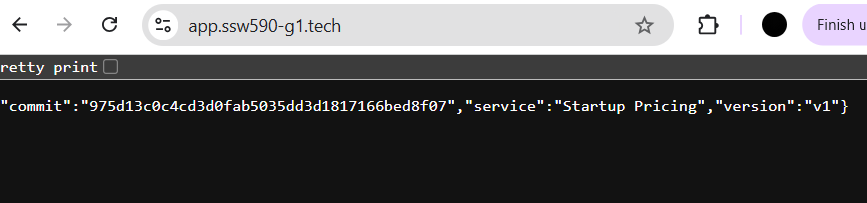
\includegraphics[width=0.9\linewidth]{evidence/234-app-root-v1-after-rollback-in-browser-bd-2026-11-18.png}
\caption{The production URL after the rollback: version v1, commit \texttt{975d13c} (BD's screenshot).}
\label{Fig:E234}
\end{figure}

\begin{longlisting}
\inputminted[fontsize=\scriptsize]{text}{evidence/237-staging-failed-deploy-injected-with-replay-manifest-unknown-bd-2026-11-18.txt}
\caption{The deliberately failed staging deployment: manifest unknown, the running container kept (real output).}
\label{Listing:E237}
\end{longlisting}

\begin{longlisting}
\inputminted[fontsize=\scriptsize]{text}{evidence/238-staging-recovered-to-v1-after-failed-deploy-bd-2026-11-18.txt}
\caption{Staging recovered to v1; the Compose file restored; times (real output).}
\label{Listing:E238}
\end{longlisting}


\begin{longlisting}
\inputminted[fontsize=\scriptsize]{text}{evidence/243-failed-deployment-drill-gunicorn-8001-staging-compose-wait-fails-bd-2026-11-18.txt}
\caption{The course's failed-deployment drill: Gunicorn on 8001 in staging, the Compose wait fails, the Jenkins run stops (real output).}
\label{Listing:E243}
\end{longlisting}

\begin{figure}[htbp]
\centering
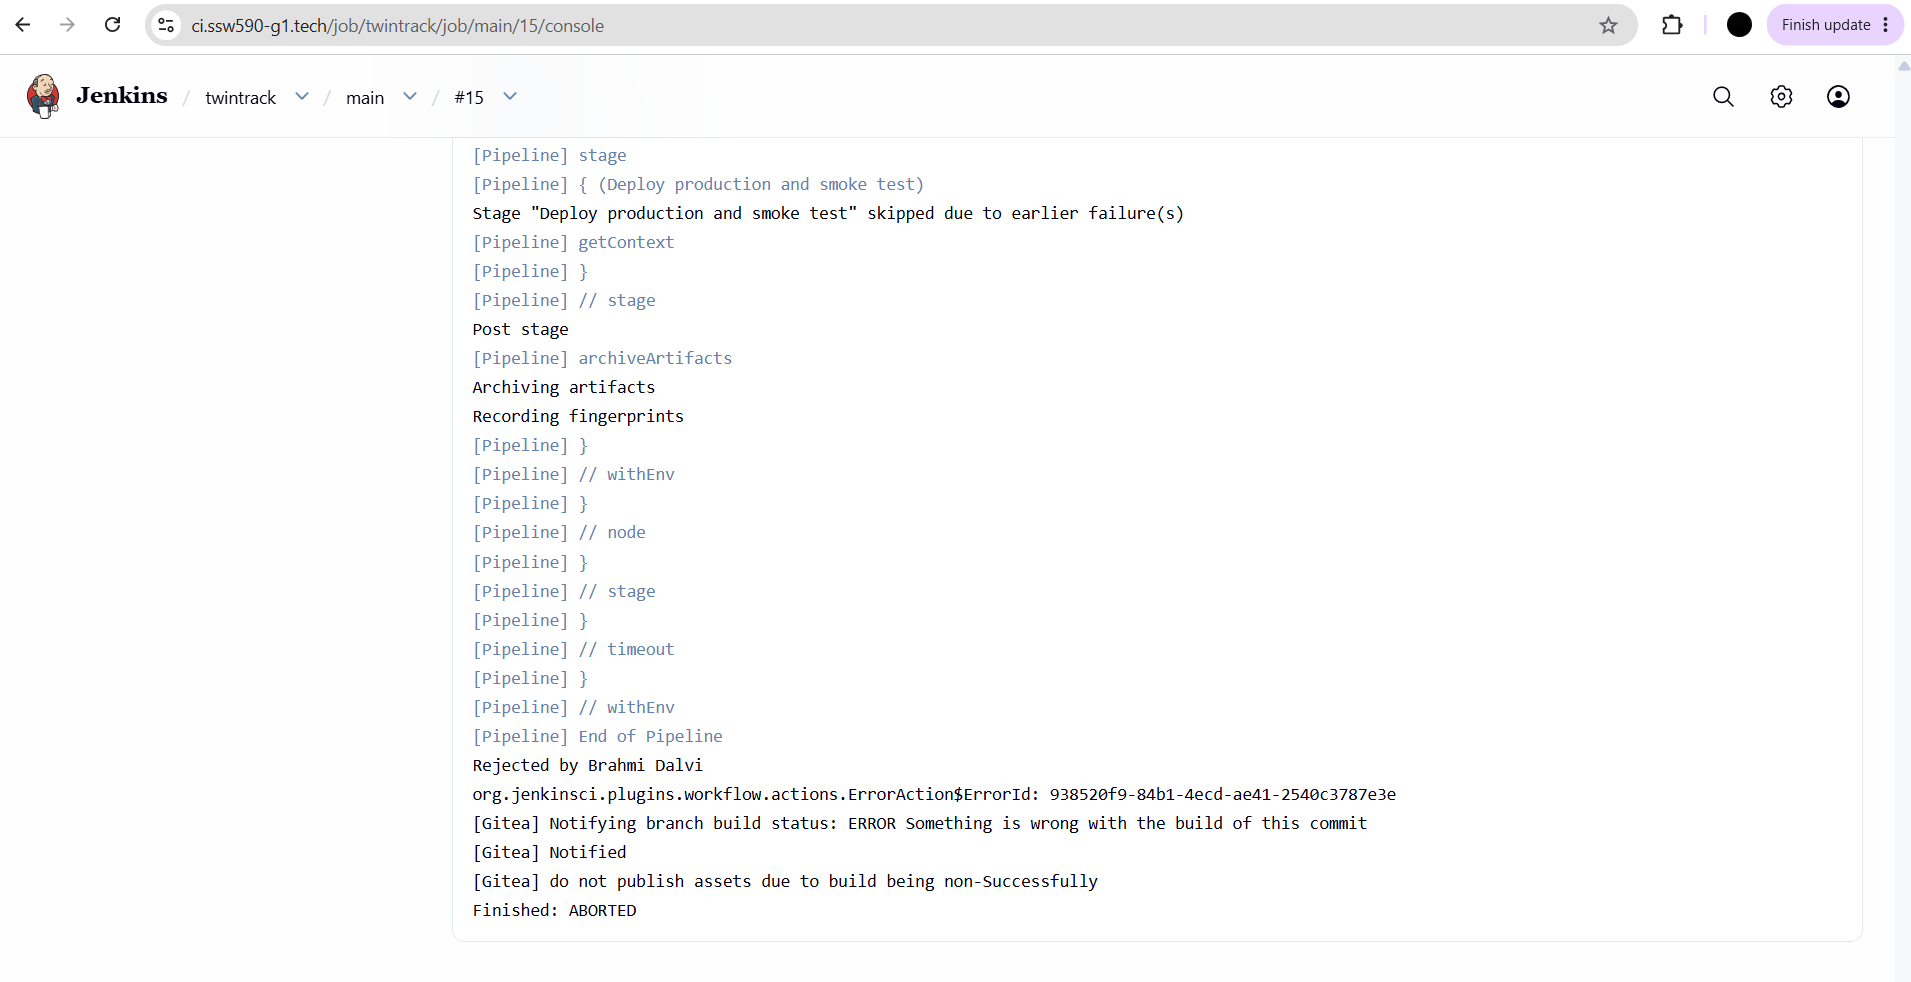
\includegraphics[width=0.9\linewidth]{evidence/244-build-15-restore-build-aborted-at-the-approval-bd-2026-11-18.png}
\caption{Jenkins build \#15, the restore build: production stage skipped, ``Rejected by Brahmi Dalvi'', aborted at the approval (BD's screenshot).}
\label{Fig:E244}
\end{figure}

\begin{longlisting}
\inputminted[fontsize=\scriptsize]{text}{evidence/245-failed-deployment-drill-restore-template-staging-healthy-again-bd-2026-11-18.txt}
\caption{The reviewed template restored through its own pull request; staging healthy on 8000 again (real output).}
\label{Listing:E245}
\end{longlisting}

\begin{longlisting}
\inputminted[fontsize=\scriptsize]{text}{evidence/246-staging-previous-release-record-reapplied-after-drill-bd-2026-11-19.txt}
\caption{The previous staging release record applied again; both environments on the known-good digest (real output).}
\label{Listing:E246}
\end{longlisting}


% ===== BD region: row 7 (5 points) =====
\section{Monitoring correlation and limits (5 points)}\label{Section:deliveryMonitoring}
\textbf{Owner:} BD. \textbf{Status:} production probe added and compared with the releases on November 17, 2026 \StatusPass; no alert reached Discord (reported by BD).

\paragraph{What was added.} The Chapter~\ref{Chapter:Sre} probe job \texttt{https} (Blackbox Exporter, module \texttt{http\_2xx}, 30~second interval) got one more target, the production health URL \texttt{https://app.ssw590-g1.tech/health}.
BD edited the live file herself: the first manual edit was rejected by \texttt{promtool} (a misplaced line and a lost indentation) and was not applied; the second, a one-line \texttt{sed} insert, passed, and Prometheus was restarted
(a single-file bind mount is not re-read on reload); \texttt{probe\_success} was 1 for all three targets (\ListRef{219}, \FigRef{220}). The existing alert rule \texttt{https-service-down} covers every target of the job, so no new rule was needed.
Staging is deliberately \emph{not} probed, so that the planned failed-deploy exercise does not trip the alert. The infrastructure repository copy of the file, together with the Jenkins controller tag and the two Caddy blocks of this assignment, was brought up to date in \texttt{infra} pull request \#8 (issue \#7), merged by BD on November 17, 2026 as merge commit \texttt{a841904}; the change only records what is already live on the server, the \texttt{infra} repository has no written review rule (the contributing rules of \texttt{CONTRIBUTING.md} belong to \texttt{twintrack}), and no review was requested (\FigRef{241}).

\paragraph{What the monitoring showed and what it did not.} Across the v2 promotion at 21:21:44~EST and the rollback at 21:23:37~EST the probe stayed at 1 (\FigRef{236}); the minimum of \texttt{probe\_success} over the previous 10 and 15 minutes was 1 when queried (\ListRef{232}).
The observer on the server saw 2 to 3 seconds without a good answer at the rollback (\ListRef{233}); the probe, with a 30~second scrape interval, never sampled it, and the alert rule, with a 1-minute pending period, cannot fire for a gap that short; BD checked the Discord alerts channel after the runs of the evening of November 17, 2026 and reported that no alert had fired (no screenshot was taken). The same blind spot holds for the 14-second restart of Jenkins (\ListRef{202}).

\paragraph{Limits.} (1) The probe answers 200 for v1 and v2: it shows availability, not whether the price is right; the Ansible smoke test, which checks version, commit and total, is the check that catches a wrong release. (2) A short rollback can fit between two scrapes and be invisible in the metrics. (3) Staging is not probed.
(4) Monitoring runs on the host it watches, so a host outage silences both. (5) The disk is the tight resource (3.5~GB free, 83\% used): the node dashboard and the existing disk alert are the monitoring for it. (6) A release does not yet leave a mark on the dashboard; the correlation is done by hand from the Jenkins times (UTC) and the Prometheus samples.

\begin{longlisting}
\inputminted[fontsize=\scriptsize]{text}{evidence/219-prometheus-probe-for-production-app-added-bd-2026-11-17.txt}
\caption{The production URL added to the probe job (real output pasted by BD).}
\label{Listing:E219}
\end{longlisting}

\begin{figure}[htbp]
\centering
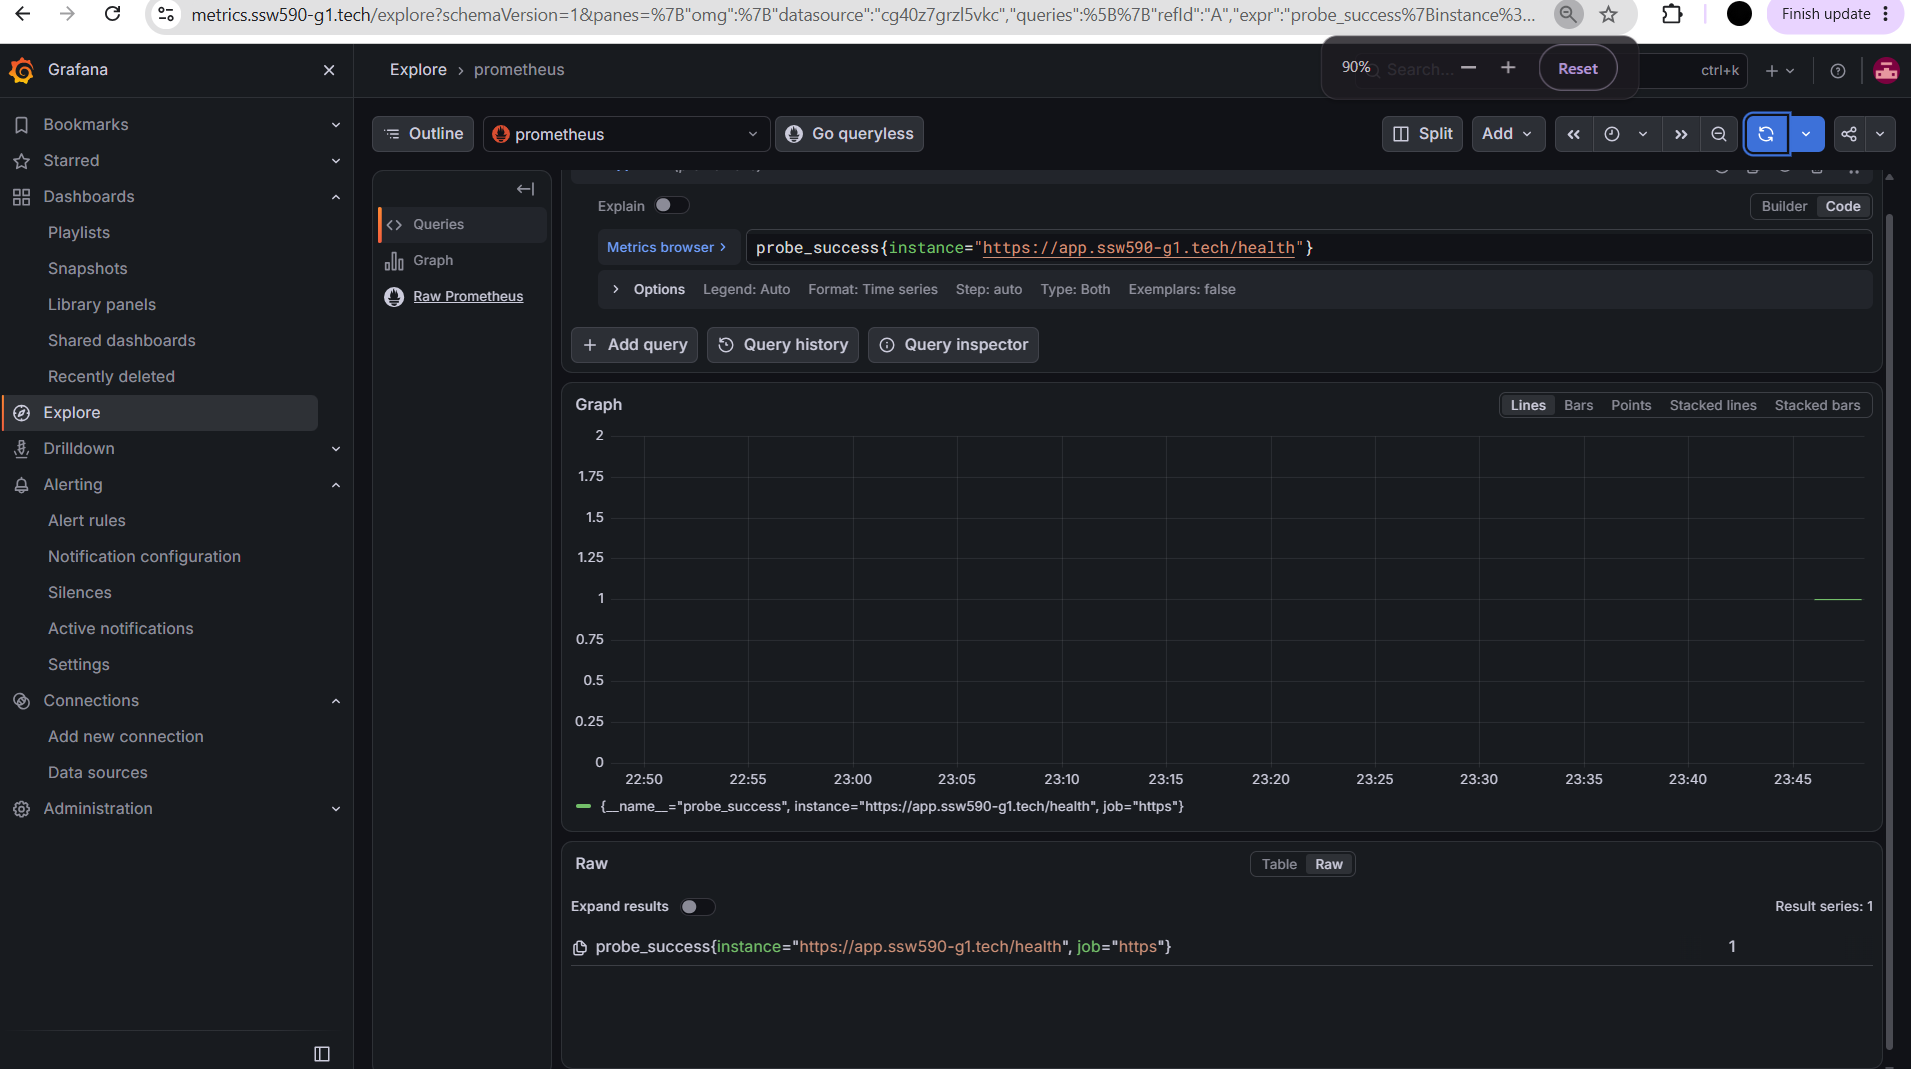
\includegraphics[width=0.9\linewidth]{evidence/220-grafana-explore-probe-success-app-health-bd-2026-11-17.png}
\caption{Grafana Explore: \texttt{probe\_success} of the production URL (BD's screenshot).}
\label{Fig:E220}
\end{figure}

\begin{figure}[htbp]
\centering
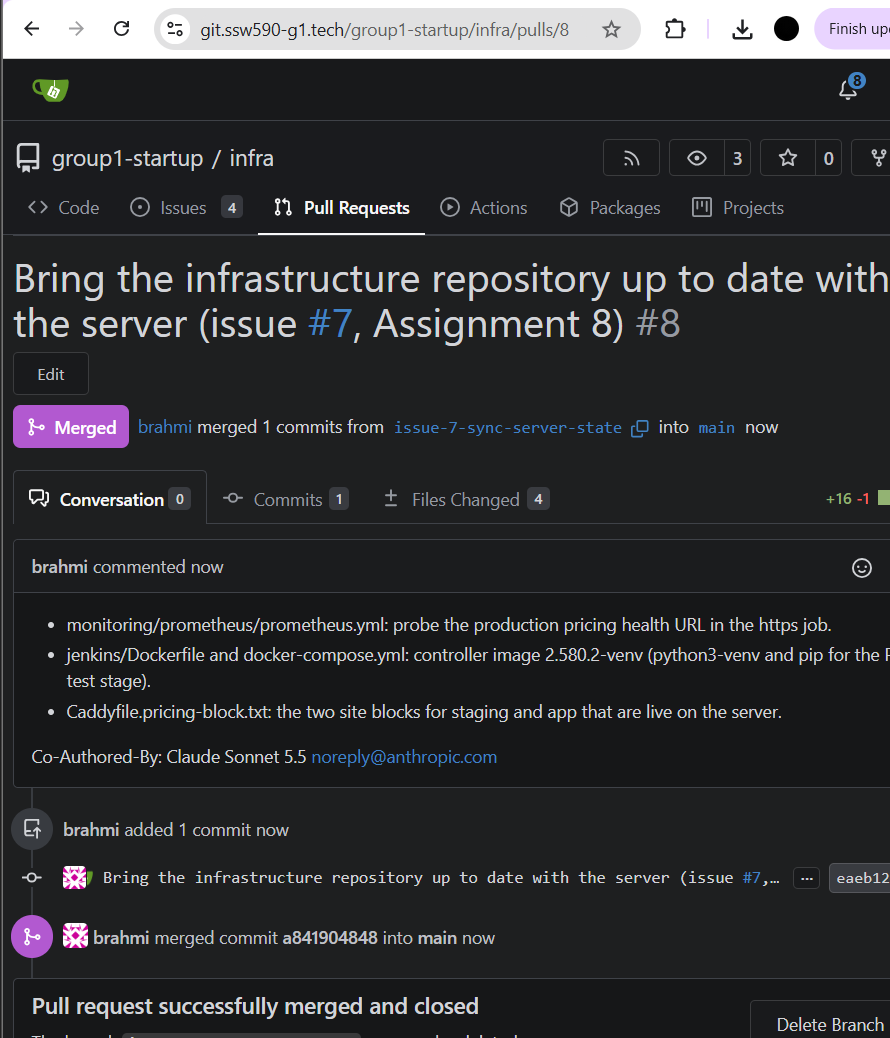
\includegraphics[width=0.9\linewidth]{evidence/241-infra-pr-8-merged-sync-with-server-bd-2026-11-18.png}
\caption{Pull request \#8 of the \texttt{infra} repository, merged: the repository matches the server again (BD's screenshot).}
\label{Fig:E241}
\end{figure}

\begin{figure}[htbp]
\centering
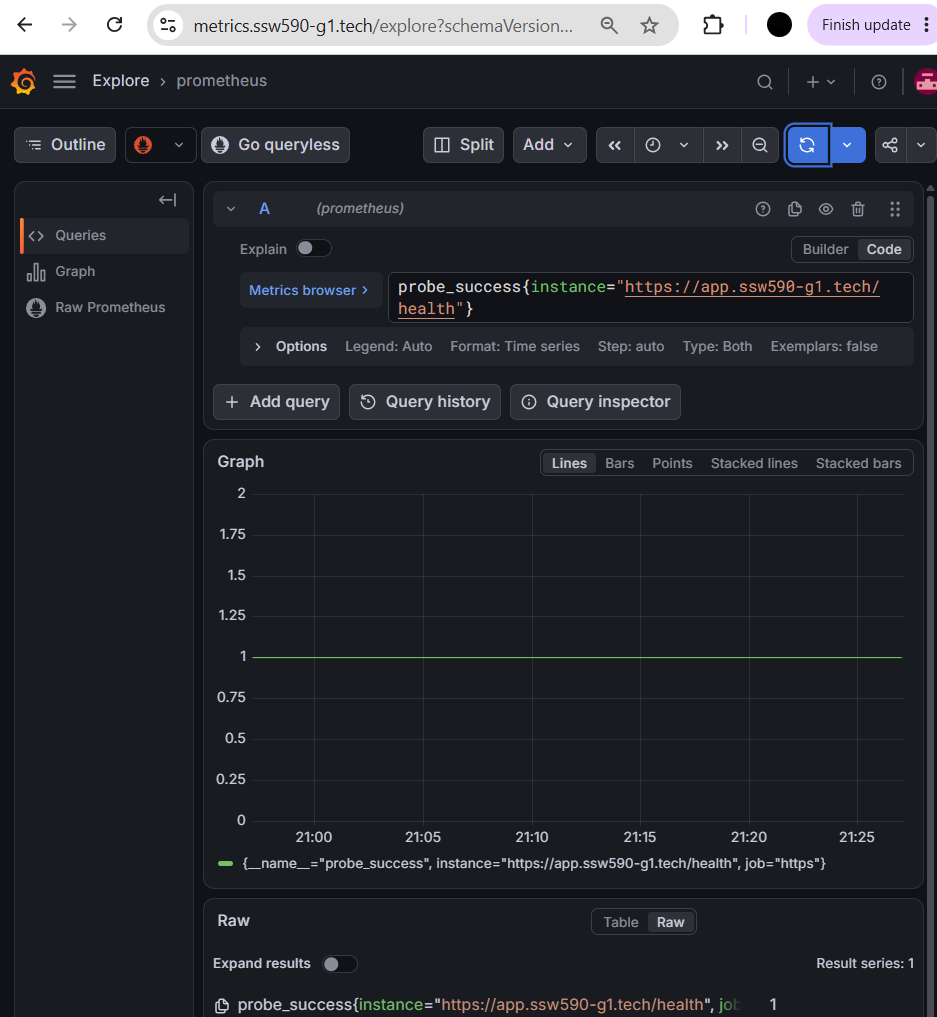
\includegraphics[width=0.9\linewidth]{evidence/236-grafana-explore-probe-success-app-flat-1-through-rollback-bd-2026-11-18.png}
\caption{The probe stays at 1 across the v2 promotion and the rollback (BD's screenshot).}
\label{Fig:E236}
\end{figure}

